\documentclass[a4paper,12pt]{article}
\usepackage[utf8]{inputenc}
\usepackage{mathtools}
\usepackage{framed}
\usepackage{epstopdf}
\usepackage[spanish]{babel}
\usepackage{appendix}
\usepackage[usenames,dvipsnames,table]{xcolor}
\usepackage{minted}
\usepackage[a4paper]{geometry}

\renewcommand{\appendixname}{Apéndices}
\renewcommand{\appendixtocname}{Apéndices}
\renewcommand{\appendixpagename}{Apéndices}

\newminted{vhdl}{mathescape, linenos, numbersep=15pt, frame=lines,framesep=2mm}
               
\newminted{matlab}{mathescape, linenos, numbersep=15pt, frame=lines,framesep=2mm}               

\definecolor{bg}{rgb}{0.95,0.95,0.95}


% Allow the change of line spacing
\usepackage{setspace}
\usepackage{tabularx}
\usepackage{graphicx}


%\usepackage{hyperref}
%\usepackage{breakurl}

%opening
%\title{Trainmining}
%\author{Grupo de Sistemas Inteligentes \\ Universidad Politécnica de Madrid}


\begin{document}
\newcommand\litem[1]{\item{\bfseries #1 }}
\renewcommand{\arraystretch}{1.5} %Makes tables less crammed

\newcommand\headcell[1]{%
  \multicolumn{1}{c|}{\cellcolor{MidnightBlue}\bfseries\sffamily\textcolor{white}{#1}}
}
\newcommand\headcelld[1]{%
  \multicolumn{1}{c||}{\cellcolor{MidnightBlue}\bfseries\sffamily\textcolor{white}{#1}}
}

%\renewcommand{\abstractname}{Executive Summary}
%\begin{abstract}
%
%\end{abstract}

% Set line spacing to 1.5
%\onehalfspacing

% Begin a new titlepage. Tit	lepages have special settings like the absence of page numbers.
\begin{titlepage}
\sffamily
% Set the text of the page to right-aligned until \end{flushright}
\begin{flushright}

% Set the space between right page border and text to 2.5cm
\rightskip=-0cm

% Show an image at this position 
%\includegraphics[bb=0 0 204 110]{web40logo.png}

% Skip a little space
\vspace*{3cm}


% Create a title for the document and write it in bold font
\huge{\textbf{DCSE - Grupo especial}}
% Again, do a line break
\linebreak
% Create a subtitle
\LARGE{Trabajo con herramientas de diseño CAD-VHDL.}

% Skip some space
\vspace*{10cm}




\large{Memoria del proyecto}
\linebreak
\normalsize{Madrid, Noviembre 2012}

% Skip some space
\vspace*{3cm}


% Provide some author information
\normalsize{Autor:}
\linebreak
\large{Adrián Pérez Orozco}
\linebreak

% End right-alignment at this point
\end{flushright}
% End the title page
\end{titlepage}

%\maketitle

\newpage
\tableofcontents % indice de contenidos
\addcontentsline{toc}{section}{Contenidos} % para que aparezca en el indice de 

\section{Introducción}
En esta memoria vamos a tratar un proyecto realizado para la asignatura \emph{Diseño de Circuitos y Sistemas Electrónicos} impartida en la ETSI de Telecomunicación de la Universidad Politécnica de Madrid.

El proyecto se propone como trabajo adicional a la asignatura, para tratar los temas de diseño de circuitos digitales de una forma más práctica y obtener conocimientos mucho más amplios sobre tecnologías relacionadas con estos campos.

En concreto, la propuesta consiste en el diseño y simulación de un sistema utilizando VHDL. El sistema propuesto consiste en un ecualizador de audio, del cual se implementarán algunos subsistemas de procesado digital en VHDL. Esta práctica se apoya sobre el trabajo realizado en el año anterior en el \emph{Laboratorio de Sistemas Electrónicos Digitales}, donde se realizó este sistema utilizando un microcontrolador.

El esquema de dicho sistema puede verse en la figura~\ref{fig:sysdesc}. El proyecto que nos ocupa se centrará en la realización del subsistema de procesado digital de audio, cuyo esquema puede verse en la figura~\ref{fig:digproc}.

Para la realización del proyecto se ha utilizado la herramienta ModelSim. De forma auxiliar, se utilizará la herramienta MATLAB para el tratamiento de las señales obtenidas de forma sencilla y eficiente, para poder así evaluar el funcionamiento del sistema.

\begin{figure}[hbt]
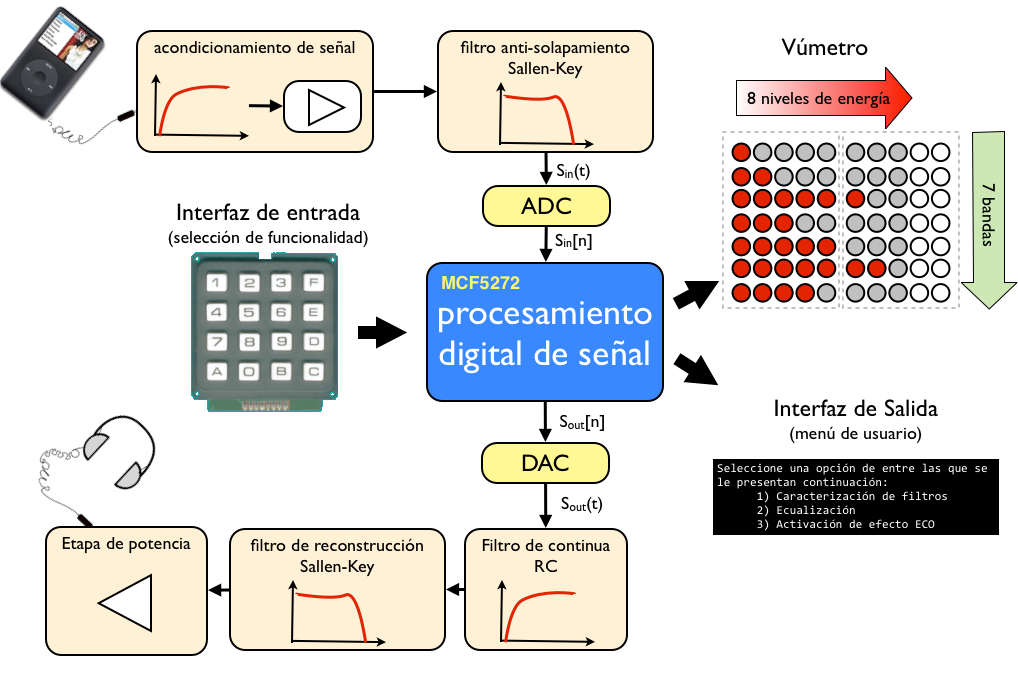
\includegraphics[width=\textwidth]{img/system_description.png} 
\caption{Descripcción del sistema completo} \label{fig:sysdesc}
\end{figure}

\begin{figure}[hbt]
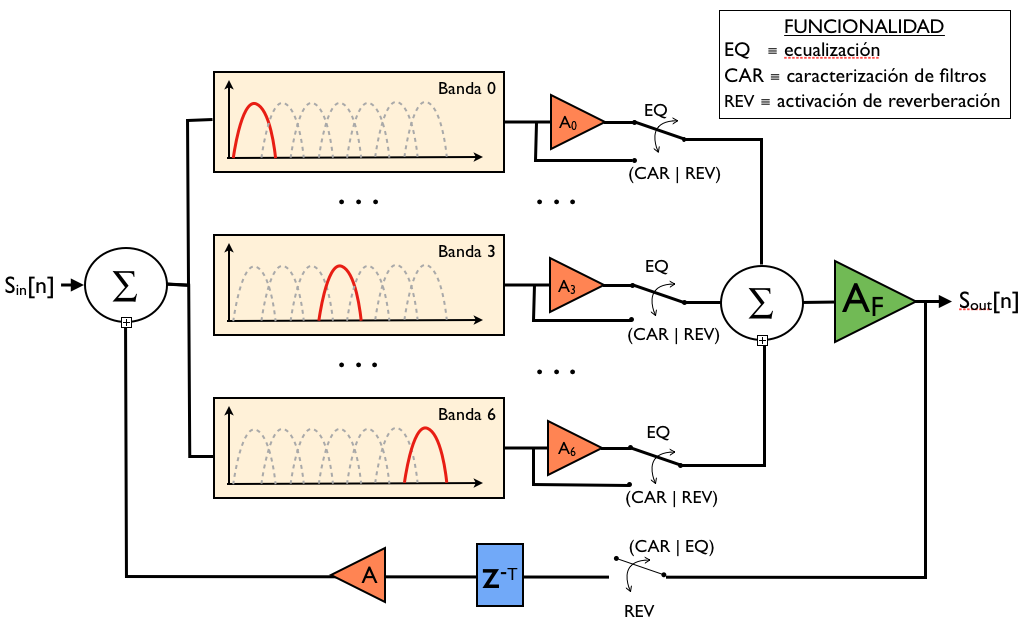
\includegraphics[width=\textwidth]{img/digital_proc.png} 
\caption{Descripcción del subsistema de procesado digital} \label{fig:digproc}
\end{figure}

\subsection{Descripción de los módulos VHDL}
El subsistema digital representado en la figura~\ref{fig:digproc} se va a dividir en los siguientes módulos principales VHDL:
\begin{description}
\item[Banco de filtros] Este módulo incluye los 7 filtros digitales que separarán la señal de entrada en sus diferentes bandas de frecuencia. Incluye 7 submódulos correspondientes a los 7 filtros digitales. Además, este módulo ofrece la funcionalidad de selección de ganancia, como se explicará posteriormente.
\item[Módulo de reverberación] Este módulo sirve para retardar y atenuar una señal. Se utilizará para realimentar en el banco de filtros la salida retardada hasta la entrada, para generar un efecto de reverberación. El subsistema de retardo se ha implementado independientemente como un submódulo.
\item[Vúmetro] Proporciona información sobre el nivel de señal de cada una de las bandas de audio. Consiste en 7 elementos vúmetro individuales que se agrupan para obtener el vúmetro de 7 bandas.
\end{description}

Todo ello se ha agrupado en un único módulo \emph{ecualizador}, para facilitar la simulación y la ejecución de pruebas. La relación de módulos y señales puede verse en la figura~\ref{fig:vhdl_schema}.

Por último, se han implementado sumadores y multiplicadores con las estructuras estudiadas en clase. Como mejora, se han sustituido las operaciones de suma y multiplicación de señales en el sistema mediante funciones VHDL (operadores + y *) por sumas y productos obtenidos mediante sumadores y multiplicadores más realistas.

\begin{figure}[hbt]
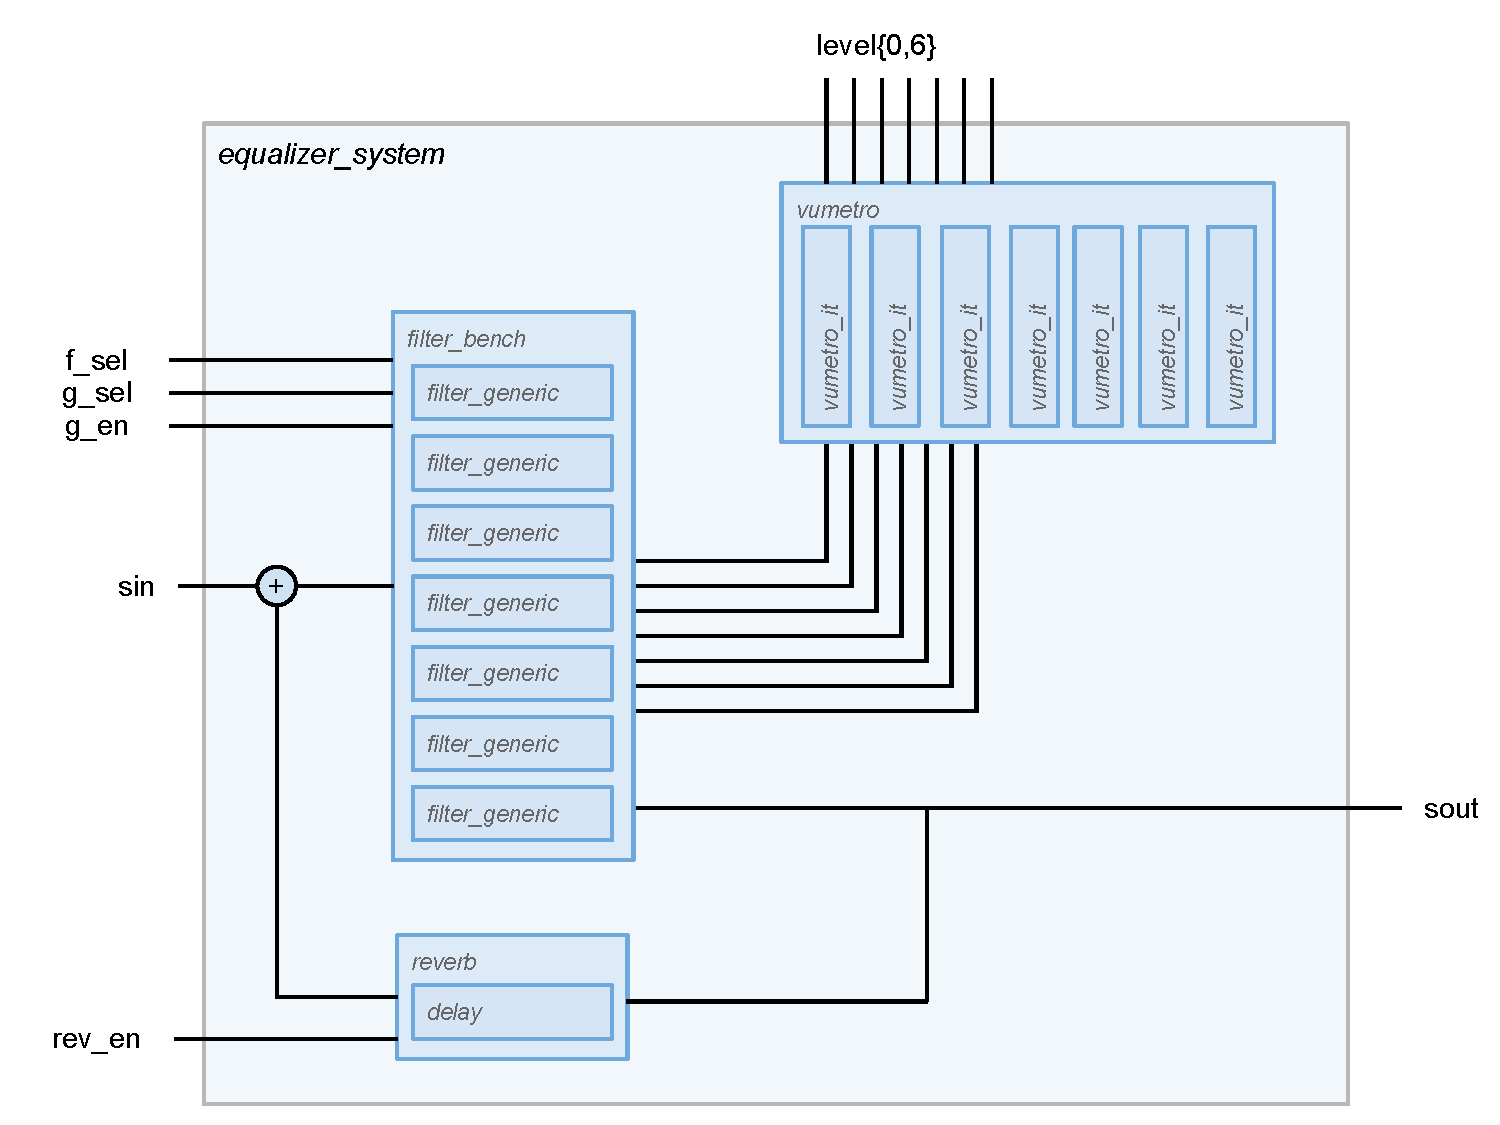
\includegraphics[width=\textwidth]{img/vhdl_schema.pdf} 
\caption{Relación de módulos VHDL} \label{fig:vhdl_schema}
\end{figure}

\clearpage
\section{Diseño de banco de filtros}
El sistema propuesto se trata de un ecualizador de audio, por lo que las señales de entrada que tendremos estarán comprendidas en el rango de frecuencias audibles por el hombre. En concreto, la especificación del sistema propuesto propone señales cuya frecuencia estará comprendida aproximadamente entre los 22 Hz y los 2.8 KHz.

Este rango de frecuencias se dividirá en 7 bandas, para lo cual utilizaremos filtros IIR de segundo orden. Las bandas de frecuencias se detallan en la tabla \ref{tab:filters}, y los coeficientes para la realización de los filtros IIR en la tabla \ref{tab:filters}.

\begin{table}
\begin{center}
 \begin{tabular}{|c||c|c|c|}
\hline 

\headcelld{Banda} & \headcell{$f_0$} & \headcell{$f_{c1}$} & \headcell{$f_{c2}$} \\ 
\hline
\hline 
0 & 31.25 & 22.10 & 44.19 \\ 
\hline 
1 & 62.5 & 44.19 & 88.39 \\ 
\hline 
2 & 125 & 88.39 & 176.78 \\ 
\hline 
3 & 250 & 176.78 & 353.55 \\ 
\hline 
4 & 500 & 323.55 & 704.11 \\ 
\hline 
5 & 1000 & 707.11 & 1414.21 \\ 
\hline 
6 & 2000 & 1414.21 & 2828.43 \\ 
\hline 
\end{tabular} 
\caption{Descripción de las distintas bandas y sus filtros asociados} \label{tab:bands}
\end{center}
\end{table}

\begin{table}
\begin{center}
 \begin{tabular}{|c||c||c|c|c||c|c|c|}
\headcelld{Filtro} & \headcelld{Ganancia} & \headcell{$a_0$} & \headcell{$a_1$} & \headcelld{$a_2$} & \headcell{$b_0$} & \headcell{$b_1$} & \headcell{$b_2$} \\ 
\hline
\hline 
0 & 8 & 1024 & -2029 & 1006 & 1024 & 0 & -1024  \\ 
\hline 
1 & 17 & 1024 & -2011 & 988 & 1024 & 0 & -1024 \\ 
\hline 
2 & 34 & 1024 & -1970 & 955 & 1024 & 0 & -1024 \\ 
\hline 
3 & 66 & 1024 & -1878 & 890 & 1024 & 0 & -1024 \\ 
\hline 
4 & 125 & 1024 & -1660 & 772 & 1024 & 0 & -1024 \\ 
\hline 
5 & 227 & 1024 & -1115 & 569 & 1024 & 0 & -1024 \\ 
\hline 
6 & 392 & 1024 & 141 & 239 & 1024 & 0 & -1024 \\ 
\hline 
\end{tabular} 
\caption{Descripción de los coeficientes de los filtros IIR} \label{tab:filters}
\end{center}
\end{table}

\subsection{Implementación de los filtros en VHDL}
Para una implementación más sencilla de los filtros, utilizaremos la \emph{Forma directa II}. El detalle de esta implementación se puede ver en la figura \ref{fig:filter_diagram}.

\begin{figure}[hbt]
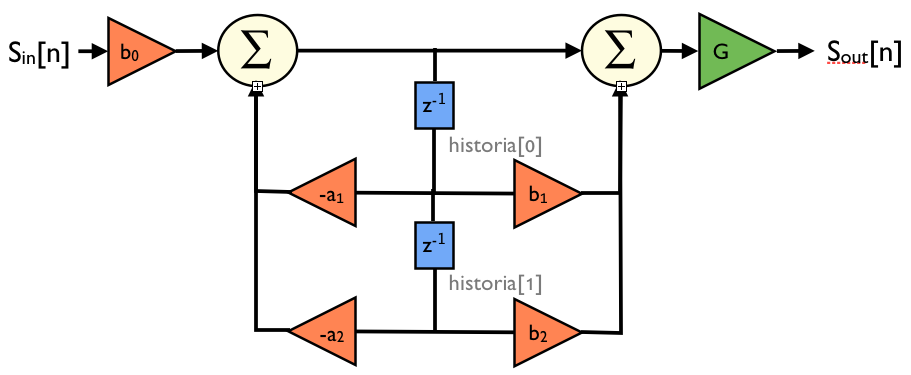
\includegraphics[width=\textwidth]{img/filter.png} 
\caption{Diagrama de bloques de un filtro IIR de segundo orden} \label{fig:filter_diagram}
\end{figure}

A la hora de implementar estos filtros digitales, tenemos que tener en cuenta una limitación muy importante. Debemos definir un ancho de palabra fijo para la representación de las señales de entrada y de salida. En nuestro caso, hemos escogido un ancho de palabra de \emph{16 bits}, correspondientes a \emph{6 bits enteros} y \emph{10 bits fraccionarios}. Esto es especialmente conveniente a la hora de representar los coeficientes de los filtros, ya que para todos ellos tenemos que $a_0 = 1024$. Normalizar los coeficientes realizando una división por 1024 equivale a desplazar los bits 10 lugares a la derecha (o lo que es lo mismo, la coma decimal 10 lugares a la izquierda). De esta forma, cuando representemos los coeficientes enteros como palabras binarias de 16 bits, bastará como tomar los 10 bits menos significativos como fraccionarios para tener el coeficiente normalizado a 1024.

\subsection{Ruido de cuantificación}
El haber elegido un ancho de palabra de 16 bits con 6 bits enteros y 10 fraccionarios nos impone una limitación considerable en cuanto a la resolución de nuestro sistema a la hora de representar señales. Sobretodo en señales de amplitud baja, tendremos un ruido de cuantificación que puede llegar a influir en el correcto funcionamiento de nuestro sistema.

Para intentar minimizar el ruido de cuantificación, se puede intentar ajustar más el numero de bits enteros, ya que las señales con las que trabajaremos estan normalizadas a 1, y a priori debería bastarnos con un bit entero y 15 fraccionarios. Este enfoque se ha intentado realizar sin éxito en la implementación, ya que aunque las señales de entrada esten normalizadas a 1, en puntos intermedios de los filtros algunas señales pueden tomar valores más altos, produciendo desbordamiento. Por ello, se ha decidido tomar una postura más conservadora y mantener la representación con 10 bits fraccionarios, que aunque no es óptima en sentido del ruido de cuantificación, nos ofrece mayor seguridad frente a desbordamiento.

Otra forma de abordar este problema sería utilizar palabras de 32 bits en lugar de 16. Esto nos ofrecería una resolución enormemente mayor, mejorando sensiblemente la calidad del sistema. No obstante, trabajar con palabras de 32 bits supone una complejidad mucho mayor a la hora de implementar los sumadores y multiplicadores vistos en clase. Debido a que el objetivo del proyecto es mayormente didáctico y no obtener una calidad de audio excepcional, se ha decidido mantener las palabras de 16 bits y asumir los efectos del ruido de cuantificación.

\subsection{Ajuste de ganancias}
Además de separar la señal en 7 bandas de frecuencias, el banco de filtros de nuestro sistema debe aplicar a cada uno una ganancia ajustable y disponer a la salida de la señal global sumada.

La selección de ganancia para cada banda se realiza mediante 3 entradas adicionales:
\begin{description}
\item[Entrada f\_sel] Entrada de 3 bits mediante la cual seleccionamos el filtro (de 0 a 6) cuya ganancia queremos ajustar.
\item[Entrada g\_sel] Entrada de 4 bits mediante la cual seleccionamos la ganancia que queremos aplicar al filtro seleccionado. Estas ganancias se encuentran definidas en el propio sistema en forma de tabla, de forma que a cada uno de los valores 0 a 15 le corresponde un valor de ganancia predefinido.
\item[Entrada g\_en] Señal de \emph{enable} del sistema de selección de ganancia. Cuando se detecta un flanco de subida se aplica la ganancia seleccionada al filtro seleccionado.
\end{description}

Para evitar desbordamiento en la señal al aplicar la ganancia, trabajaremos con posibles valores de ganancia menores que 1 (atenuaremos la señal). De esta forma, la ganancia numero 0 corresponde a una ganancia de 0dB, y de ahí se irá bajando a medida que aumente el índice de la ganancia seleccionada.

\clearpage
\section{Diseño de módulo de reverberación}
El subsistema de reverberación consiste en un módulo que ofrece a la salida la señal que obtiene a la entrada con un retraso de N posiciones y aplicandole una atenuación determinada.

Para la implementación de este módulo se ha utilizado como base una cola FIFO, en la cual se va introduciendo la señal que posteriormente se va obteniendo por la salida tras N ciclos de reloj. Para ello es importante inicializar la cola para que esté llena de palabras a cero, ya que si no la primera muestra de la señal de entrada ocuparía la primera posición y sería la que se ofrecería a la salida en el siguiente ciclo de reloj.

En nuestro sistema, el numero de palabras en la cola será siempre fijo e igual al número de muestras que queramos retrasar la señal. La implementación de una cola FIFO tiene cierta complejidad derivada del hecho de que el numero de palabras en la cola es variable y puede ser impredecible, conllevando posibles problemas de desbordamiento o cola vacía. Sin embargo, puesto que el funcionamiento de nuestro retardador es mucho más predecible (llegará una muestra por cada ciclo de reloj y sacaremos una muestra por cada ciclo de reloj, resultando en un tamaño constante) podemos simplificar considerablemente este diseño.

Se ha implementado para ello el subsistema \emph{delay}, que consiste en una memoria de N posiciones (tamaño configurable mediante genéricos) con un puntero señalando a una de esas posiciones. En cada ciclo de reloj, se sacará la señal de la posición indicada por el puntero y se añadirá en su lugar la señal que llegue a la entrada. El valor del puntero se va aumentando de forma cíclica, de forma que la señal que acabamos de introducir no se sacará hasta que el puntero vuelva a apuntar a esa misma posición, es decir, tras N ciclos de reloj.

Posteriormente, la señal se atenúa mediante un valor de ganancia también configurable mediante genéricos, y se realimenta a la entrada del banco de filtros.

\section{Diseño de vúmetro}
El vúmetro ofrece información sobre el nivel de señal disponible en cada una de las bandas de señal. Para abordar la implementación de este módulo, se ha implementado un subsistema vúmetro con úna única entrada que ofrece el nivel de la señal que tenga a la entrada. Estos vúmetros individuales se agrupan en un módulo vúmetro de 7 entradas, que conectaremos a la salida de cada uno de los filtros del banco de filtros.

Cada uno de los vúmetros individuales generan a la salida una señal de 8 bits, simulando los leds que tradicionalmente se utilizan en estos sistemas. El número de bits que se pongan a 1 en la señal (leds que se iluminan) indicará el nivel de la señal en esa banda.

Para detectar el nivel de la señal, observaremos la palabra a nivel binario. Una palabra de la señal está representada de la siguiente forma:
$$X_{15} X_{14} X_{13} X_{12} X_{11} X_{10} X_{9} X_{8} X_{7} X_{6} X_{5} X_{4} X_{3} X_{2} X_{1} X_{0}$$
Definiremos cada uno de los 8 niveles de señal dividiendo los 16 bits en conjuntos de dos. Así, el nivel 0 corresponderá a todos los bits a 0, el nivel 1 se alcanzará cuando sólo los bits $X_1$ o $X_0$ estén a nivel alto, el nivel 2 si los bits $X_4$ o $X_3$ están a 1, y así sucesivamente. cada uno de estos niveles \emph{encenderá} a la salida el led correspondiente a su nivel además de todos los de los niveles anteriores.

Para tener en cuenta las posibles palabras negativas en complemento a dos, es importante tener en cuenta que debemos observar siempre el valor absoluto de las señales, ya que si no siempre obtendríamos el nivel más alto para cualquier entrada negativa.

\subsection{Mantenimiento del nivel}
Debido a las posibles variaciones rápidas de la señal, es importante que los picos a la salida del vúmetro se mantengan un mínimo tiempo para su correcta visualización.

Para implementar este comportamiento, se ha definido el siguiente procedimiento:
\begin{enumerate}
\item Se toma una muestra a la entrada y se mantiene en memoria
\item Se inicia un contador (configurable mediante genéricos) que indica el tiempo mínimo que se han de mantener los niveles a la salida
\item Si a la entrada llega alguna muestra mayor a la que tenemos en memoria, se sustituye y se reinicia el contador, comenzando el proceso desde el principio.
\item Si el contador llega a cero, se elimina la señal de memoria, permitiendo que otras señales más bajas tomen el lugar de la muestra. En este punto el pico anterior deja de mantenerse y el nivel del vúmetro puede bajar
\item La siguiente muestra entra en memoria y se reinicia el proceso
\end{enumerate}

Esto nos permite mantener de forma sencilla los niveles un mínimo de tiempo en pantalla sin perder información de posibles picos que puedan aparecer mientras estamos manteniendo la señal.

\section{Mejoras}
Para la aplicación de los conocimientos obtenidos en la asignatura \emph{Diseño de Circuitos y Sistemas Electrónicos}, se ha propuesto la realización de varias modificaciones que se corresponden con lo estudiado en la parte digital de la asignatura.

En concreto, se ha propuesto la implementación de sumadores y multiplicadores binarios, correspondiendose con las configuraciones estudiadas en clase. Estas implementaciones se han de realizar a bajo nivel, mediante la conexión y configuración de \emph{Full Adders}, ilustrando además los efectos de retardo en cada una de las distintas configuraciones.

En concreto, se han implementado las siguientes configuraciones:
\begin{itemize}
\item Sumador ripple carry
\item Sumador carry bypass
\item Multiplicador en array
\item Multiplicador carry save
\end{itemize}

Se ha supuesto para ello un retardo en los \emph{Full Adder} fijo de 1 ns, tanto en la generación de la señal de suma como en la señal de carry. Esto nos permite observar el efecto de los distintos caminos críticos en el retardo en la generación de las señales.

\subsection{Sumador Ripple Carry}
Este sumador es el más sencillo en términos de implementación. Simplemente se han conectado 16 full adders de forma secuencial de forma que el acarreo se propague de uno a otro.

En la figura~\ref{fig:ripple_carry_adder} se muestra un esquema simplificado (4 bits) de este sumador.

\begin{figure}[hbt]
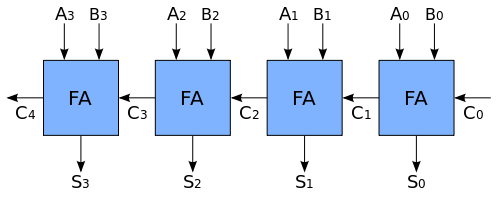
\includegraphics[width=\textwidth]{img/ripple_carry_adder.png} 
\caption{Sumador Ripple Carry de 4 bits} \label{fig:ripple_carry_adder}
\end{figure}

\subsection{Sumador Carry Bypass}
El sumador \emph{Carry Bypass} (o \emph{Carry Skip}) permite reducir el tiempo de retardo del camino crítico sensiblemente. En la figura~\ref{fig:carry_bypass_adder} puede verse un esquema de este tipo de sumador.

Para la implementación de este tipo de sumadores, se divide la operación en varios bloques. En el esquema de la figura~\ref{fig:carry_bypass_adder} estos bloques son de 4 bits, aunque se puede variar el tamaño de los mismos para optimizar aún más el retardo de este sumador.

En la figura~\ref{fig:carry_skip_block} puede verse un detalle de los bloques carry bypass.

\begin{figure}[hbt]
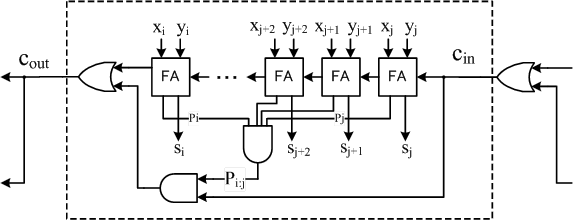
\includegraphics[width=\textwidth]{img/carryskipblock.png} 
\caption{Bloque carry bypass} \label{fig:carry_skip_block}
\end{figure}

En nuestro diseño, se ha optado por un tamaño de bloque de 4 bits, lo que resulta en un total de 4 bloques carry bypass para obtener el sumador completo. Para trabajar con las señales P y G que se han explicado en teoría, se ha implementado una versión modificada del full adder que trabaja con las señales P y G en lugar de los sumandos originales.
\clearpage
\subsection{Multiplicador en array}
El multiplicador en array corresponde a la implementación más directa de una multiplicación binaria. Para ello, simplemente se generan los productos parciales y se van sumando en distintas filas de sumadores. Esto conlleva un retardo considerablemente alto, que como podremos ver, se puede reducir mediante otras configuraciones de multiplicadores.

En la figura~\ref{fig:array_multiplier} se puede ver un esquema general de un multiplicador en array. Para un multiplicador de 16 x 16 bits como el que necesitamos en nuestro sistema, tendríamos que utilizar un total de 256 full adders. Debido a que esta cantidad es inmanejable a la hora de realizar conexiones de señales en VHDL, se ha optado por dividir la estructura del multiplicador en filas de 16 full adders, de forma que solo tengamos que diseñar una fila y después tratar con 16 filas. El diseño de estas filas (\emph{bloques de multiplicador en array}) puede verse en la figura~\ref{fig:array_multiplier_block}. Es importante destacar que esta agrupación en filas no conlleva ninguna modificación en el funcionamiento del multiplicador, y que equivale exactamente a haber conectado entre si los 256 full adders en un único módulo.

Para realizar multiplicaciones con signo, se calcula previamente el signo del resultado mediante un XOR de los MSB de los factores. Posteriormente se realiza la multiplicación del valor absoluto de los factores, invirtiendose posteriormente el signo del resultado si se espera un resultado negativo.

\begin{figure}[hbt]
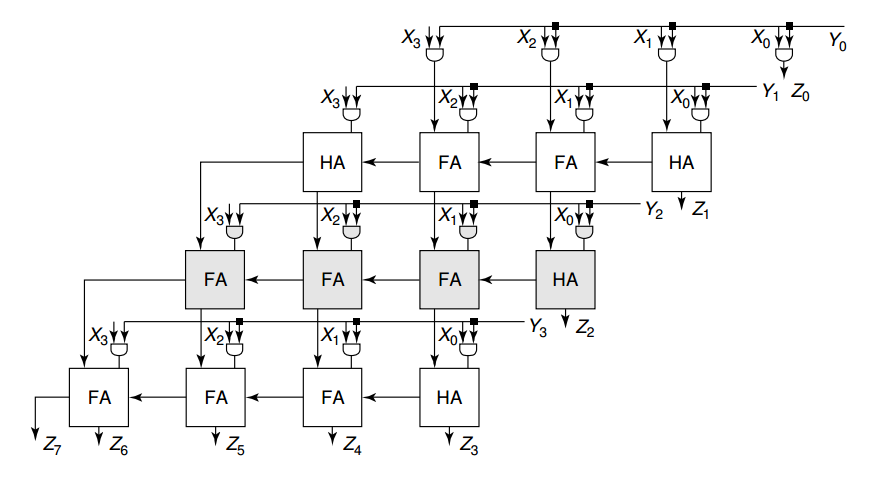
\includegraphics[width=\textwidth]{img/array_multiplier.png} 
\caption{Multiplicador en array} \label{fig:array_multiplier}
\end{figure}

\begin{figure}[hbt]
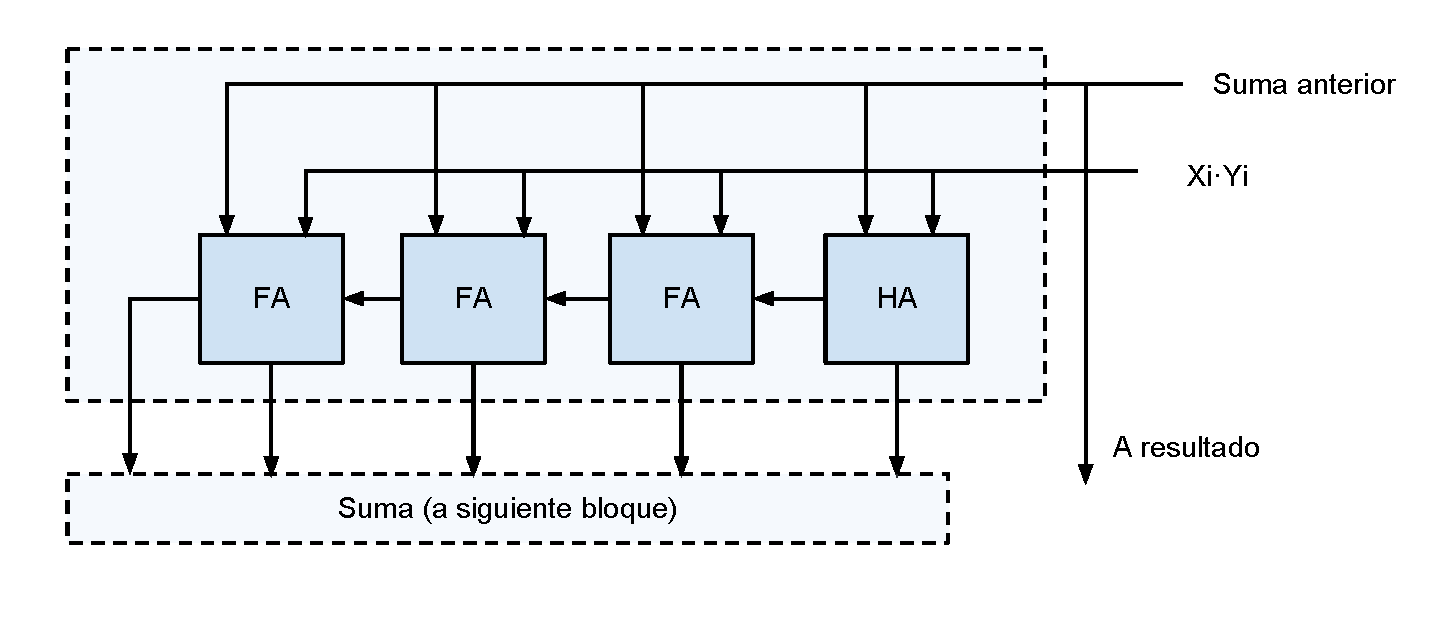
\includegraphics[width=\textwidth]{img/array_mult_block.pdf} 
\caption{Bloque de multiplicador en array} \label{fig:array_multiplier_block}
\end{figure}

\clearpage
\subsection{Multiplicador carry save}
El multiplicador carry save es una estrucutra de multiplicador modificada que permite reducir el tiempo de retardo en la generación del producto. Para ello, los acarreos de una fila de full adders no son propagados dentro de una misma fila, sino que se propagan a la fila siguiente como un sumando adicional.

El esquema de este tipo de multiplicador puede verse en la figura~\ref{fig:carry_save_multiplier}.

\begin{figure}[hbt]
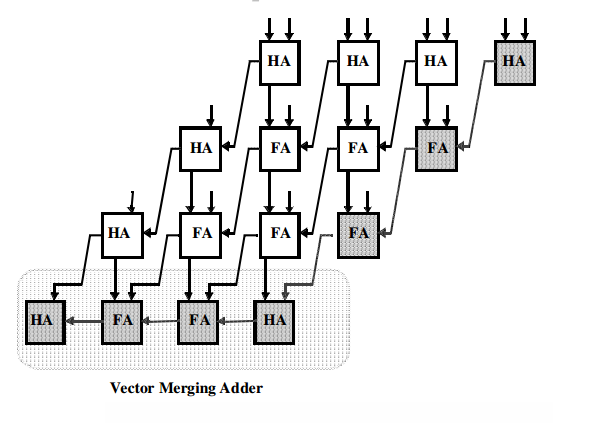
\includegraphics[width=\textwidth]{img/carry_save_mult.png} 
\caption{Multiplicador carry save} \label{fig:carry_save_multiplier}
\end{figure}

De forma análoga a lo que sucede con el multiplicador en array, realizar un multiplicador carry save de 16x16 bits conlleva la utilización de un número inmanejable de full adders. Para evitar este problema, se ha optado por una solución similar a la tomada para la implementación del multiplicador en array: dividir el sistema en bloques para cada fila de full adders.

El diseño elegido para estos bloques puede verse en la figura~\ref{fig:carry_save_block}

Para realizar multiplicaciones con signo, se calcula previamente el signo del resultado mediante un XOR de los MSB de los factores. Posteriormente se realiza la multiplicación del valor absoluto de los factores, invirtiendose posteriormente el signo del resultado si se espera un resultado negativo.

\begin{figure}[hbt]
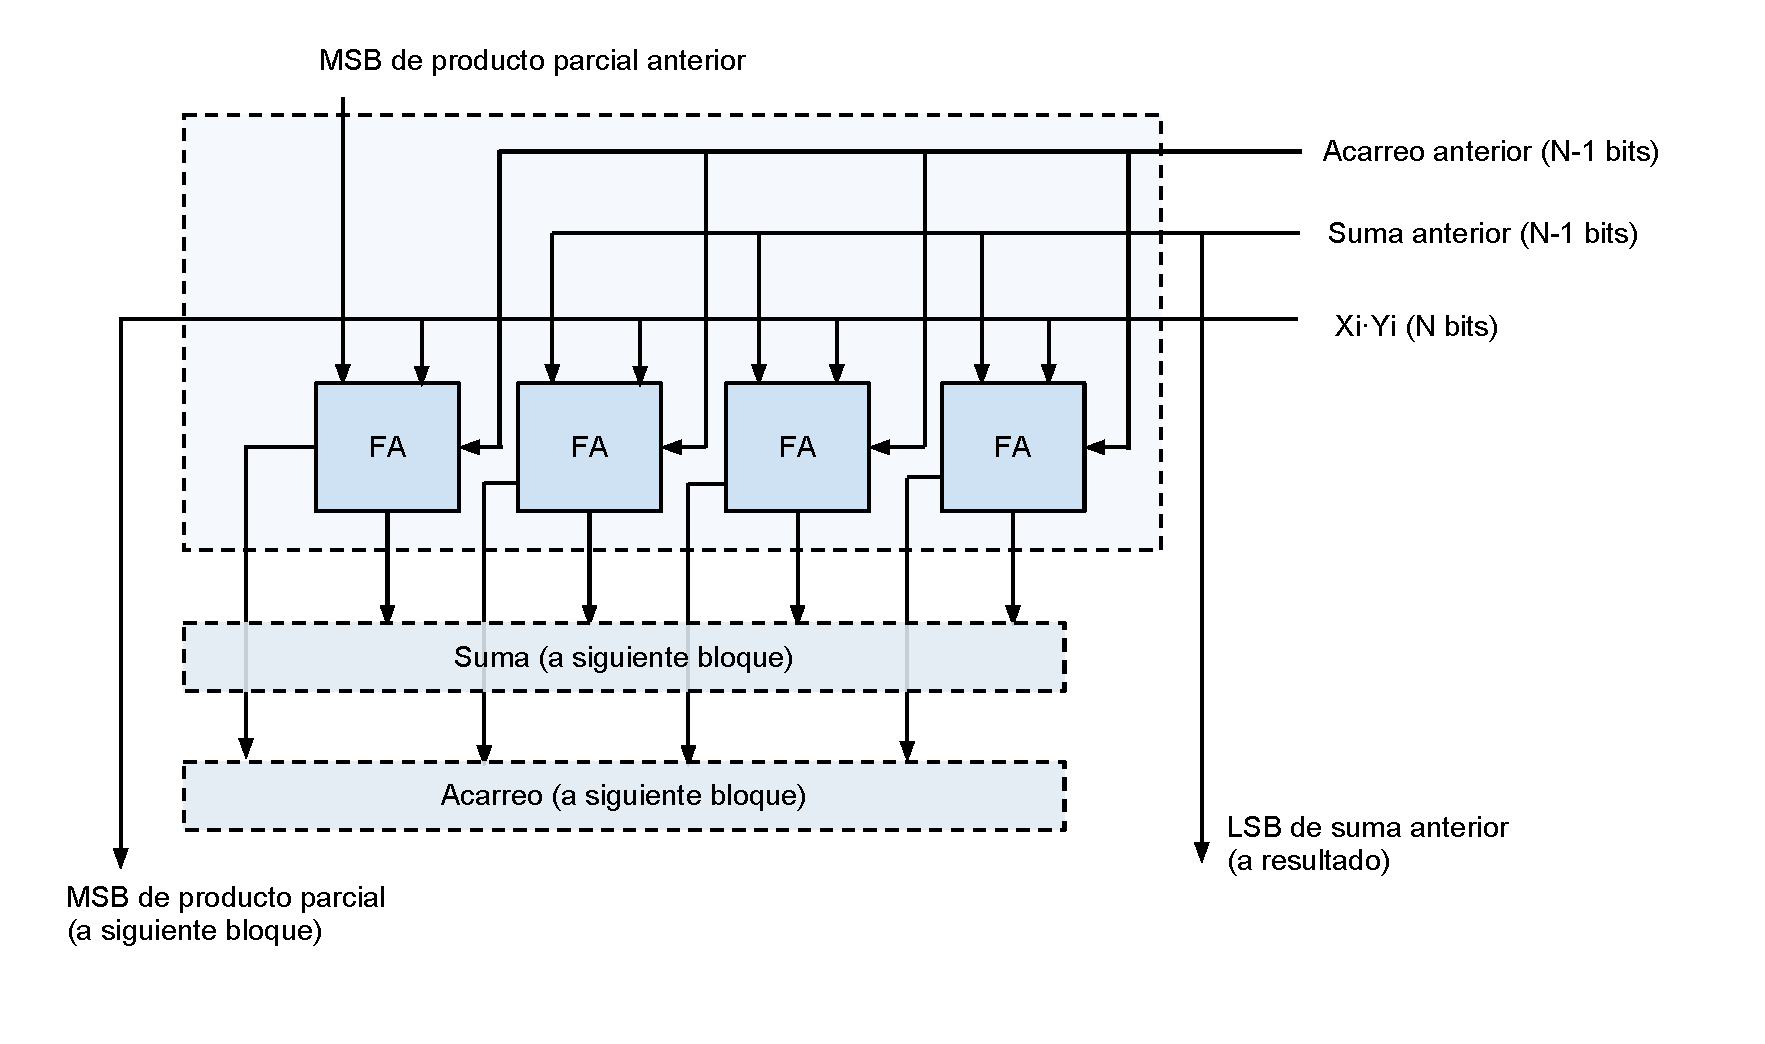
\includegraphics[width=\textwidth]{img/carry_save_block.pdf} 
\caption{Bloque del multiplicador carry save} \label{fig:carry_save_block}
\end{figure}

\clearpage
\section{Pruebas y resultados}
En esta sección se van a describir los procedimientos utilizados para evaluar el funcionamiento de los sistemas implementados
\subsection{Comprobación del funcionamiento de los filtros}\label{sec:pruebafiltros}
Para comprobar el correcto funcionamiento de los filtros, se ha comparado la respuesta al impulso obtenida en la simulación del sistema VHDL con la respuesta al impulso teórica que debería tener un filtro IIR con los coeficientes indicados en las especificaciones.

Es importante tener en cuenta que al aplicar la atenuación a la salida de los filtros (para que todas las bandas presenten una ganancia de 0dB) se aumenta considerablemente el ruido de cuantificación de la señal de salida. Para evitar este efecto a la hora de comprobar la correcta realización del filtro, se van a comparar las respuestas al impulso sin aplicar la atenuación en primer lugar, y posteriormente aplicándola.

Las gráficas detalladas con los resultados de esta prueba se encuentran en el apéndice~\ref{sec:resultadosfiltros}.

Observando los resultados, se puede ver que las respuestas al impulso que se observa sin atenuar la salida de los filtros corresponde bastante bien con la respuesta teórica esperada (calculada con MATLAB). No obstante, si observamos las respuestas al impulso con la salida atenuada, vemos que el ruido de cuantificación es considerablemente alto, especialmente en los filtros de frecuencias bajas.

Debido a que esta atenuación se aplica a la entrada (para evitar saturación en puntos intermedios) este ruido nos afecta también a los valores de realimentación dentro de la estructura del filtro, lo que nos modifica la forma de la respuesta al impulso en los filtros 0 y 1.

El diseño de los filtros es correcto, como se observa en las respuestas al impulso sin atenuar. El funcionamiento pobre de los filtros 0 y 1 se debe por tanto únicamente al error de cuantificación, y por tanto para mejorar el funcionamiento en este aspecto debería trabajarse con un mayor tamaño de palabra.


\subsection{Prueba de la función de reverb}
Para comprobar el funcionamiento de la función de reverb se ha realizado una prueba sencilla. Se ha generado un estímulo de entrada de corta duración (un periodo de una señal sinusoidal) y se ha ajustado el número de muestras del retardo de reverberación para que el \emph{eco} se produzca justo después de finalizar la señal original, pudiendo así apreciarse mejor.

Se ha comparado la señal obtenida con la función de reverb activada con la obtenida con la función de reverb desactivada. Mientras que en la señal filtrada sin reverb se pueden apreciar únicamente pequeñas oscilaciones derivadas de la respuesta de los filtros tras el ciclo sinusoidal de la señal original, en la señal con reverb se pueden apreciar claramente réplicas atenuadas de este ciclo a lo largo del tiempo.

Las gráficas que muestran este resultado pueden verse en el apéndice~\ref{sec:resultadosreverb}.


\subsection{Prueba de ajuste de ganancia}
Para comprobar el funcionamiento de la función de ajuste de ganancia se ha observado la evolución de la señal de salida mientras se va modificando la ganancia. Para ilustrar este funcionamiento, se ha tomado una señal sinusoidal centrada en la frecuencia del filtro 3, y se ha ido aumentando la atenuación progresivamente en las bandas 2, 3 y 4. En la salida puede verse claramente como la señal va atenuandose a medida que vamos variando la ganancia.

Observar de forma gráfica la evaluación temporal de la señal es la forma más adecuada de comprobar este funcionamiento. Las gráficas que muestran este resultado pueden verse en el apéndice~\ref{sec:resultadosajuste}.

\subsection{Prueba de mejoras}
Para comprobar el funcionamiento de los sumadores y multiplicadores se han realizado varias operaciones y se ha comparado el resultado que ofrecían nuestros sumadores y multiplicadores con el que resultaría de utilizar las funciones + y * de VHDL. Se pretende así comprobar que el uso de nuestros bloques operacionales corresponde exactamente al uso de las funciones VHDL. Para ello se ha elegido un conjunto de señales de prueba a sumar, teniendo cuidado en comprobar las operaciones con señales negativas.

Los resultados son satisfactorios y se obtienen en todo caso los valores esperados.

En las gráficas incluidas en el apéndice~\ref{sec:resultadosmejoras} puede observarse la comparación de estas señales.

\subsubsection*{Observación sobre retardos}
Como es de esperar, al utilizar nuestros sumadores y multiplicadores implementados con Full Adders con retardo, observamos los efectos de la propagación de las señales de suma y de acarreo. Esto se traduce en una oscilación en los valores del resultado que ofrecen nuestros bloques, que tarda unos nanosegundos en estabilizarse y ofrecer el valor correcto.

Este efecto se elimina del resto del sistema mediante el uso de una señal de reloj. Utilizando un periodo de reloj mayor que el necesario para la generación de las sumas y multiplicaciones evitamos estas oscilaciones. En la simulación se ha establecido un periodo de reloj de 100ns, suficientemente alto ya que el retardo de los full adders es de 1 ns.

En las gráficas incluidas en el apéndice~\ref{sec:resultadosmejoras} puede además verse la diferencia en el retardo de las diferentes configuraciones. Así, observamos como el sumador ripple carry en muchas ocasiones tarda sensiblemente más en estabilizar su resultado que el sumador carry bypass. También se observa esta diferencia en los multiplicadores. El multiplicador carry save tiene un retardo sensiblemente mejor que el del multiplicador en array. Esto corresponde con lo estudiado en teoría en clase.

\appendix
\clearpage
\addappheadtotoc
\appendixpage
\section{Gráficas de evaluación de filtros}\label{sec:resultadosfiltros}
Estas gráficas corresponden a los resultados de los procedimientos descritos en la sección~\ref{sec:pruebafiltros}
\subsection{Sin aplicar atenuación}
\begin{figure}[hbt]
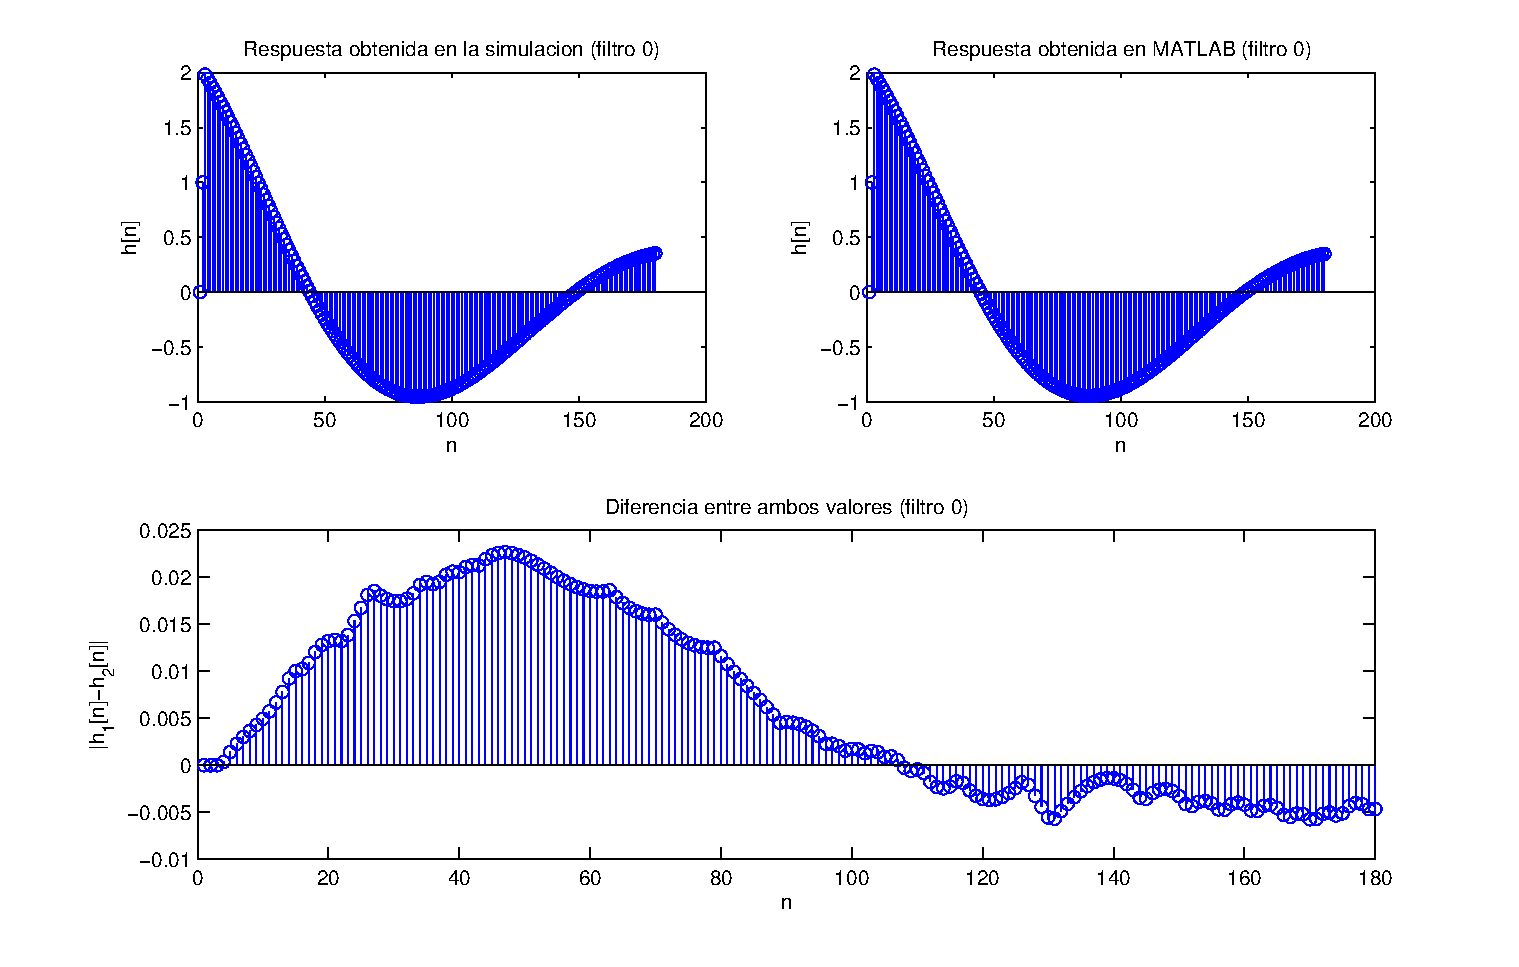
\includegraphics[width=\textwidth]{img/respfiltro0.pdf} 
\caption{Comprobación del filtro 0} \label{fig:filter0}
\end{figure}

\begin{figure}[hbt]
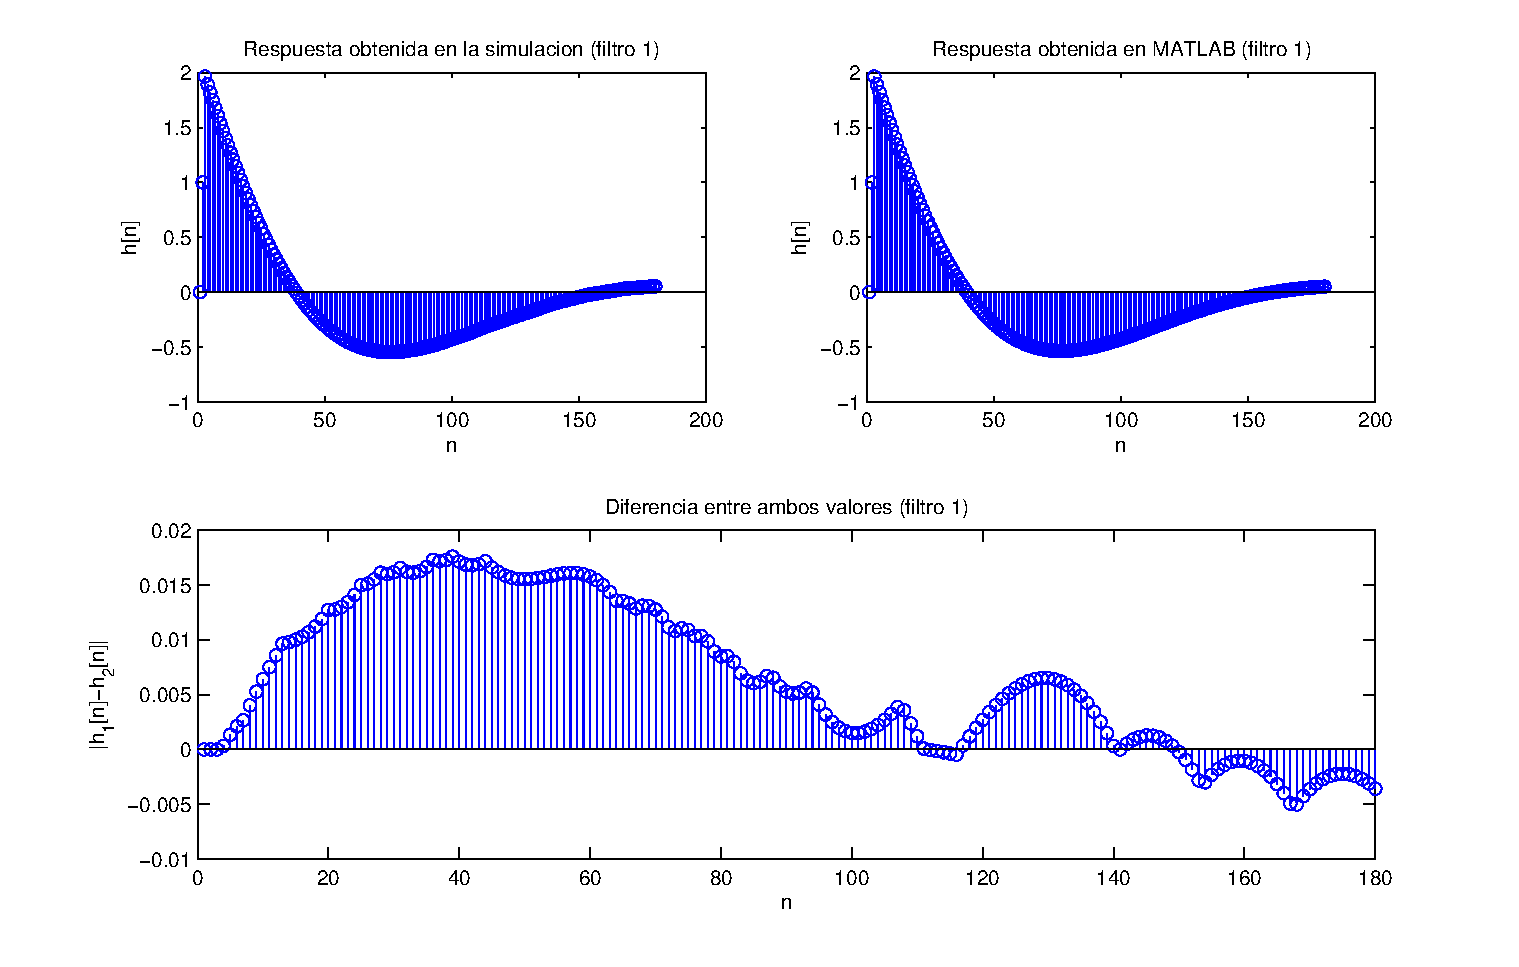
\includegraphics[width=\textwidth]{img/respfiltro1.pdf} 
\caption{Comprobación del filtro 1} \label{fig:filter1}
\end{figure}

\begin{figure}[hbt]
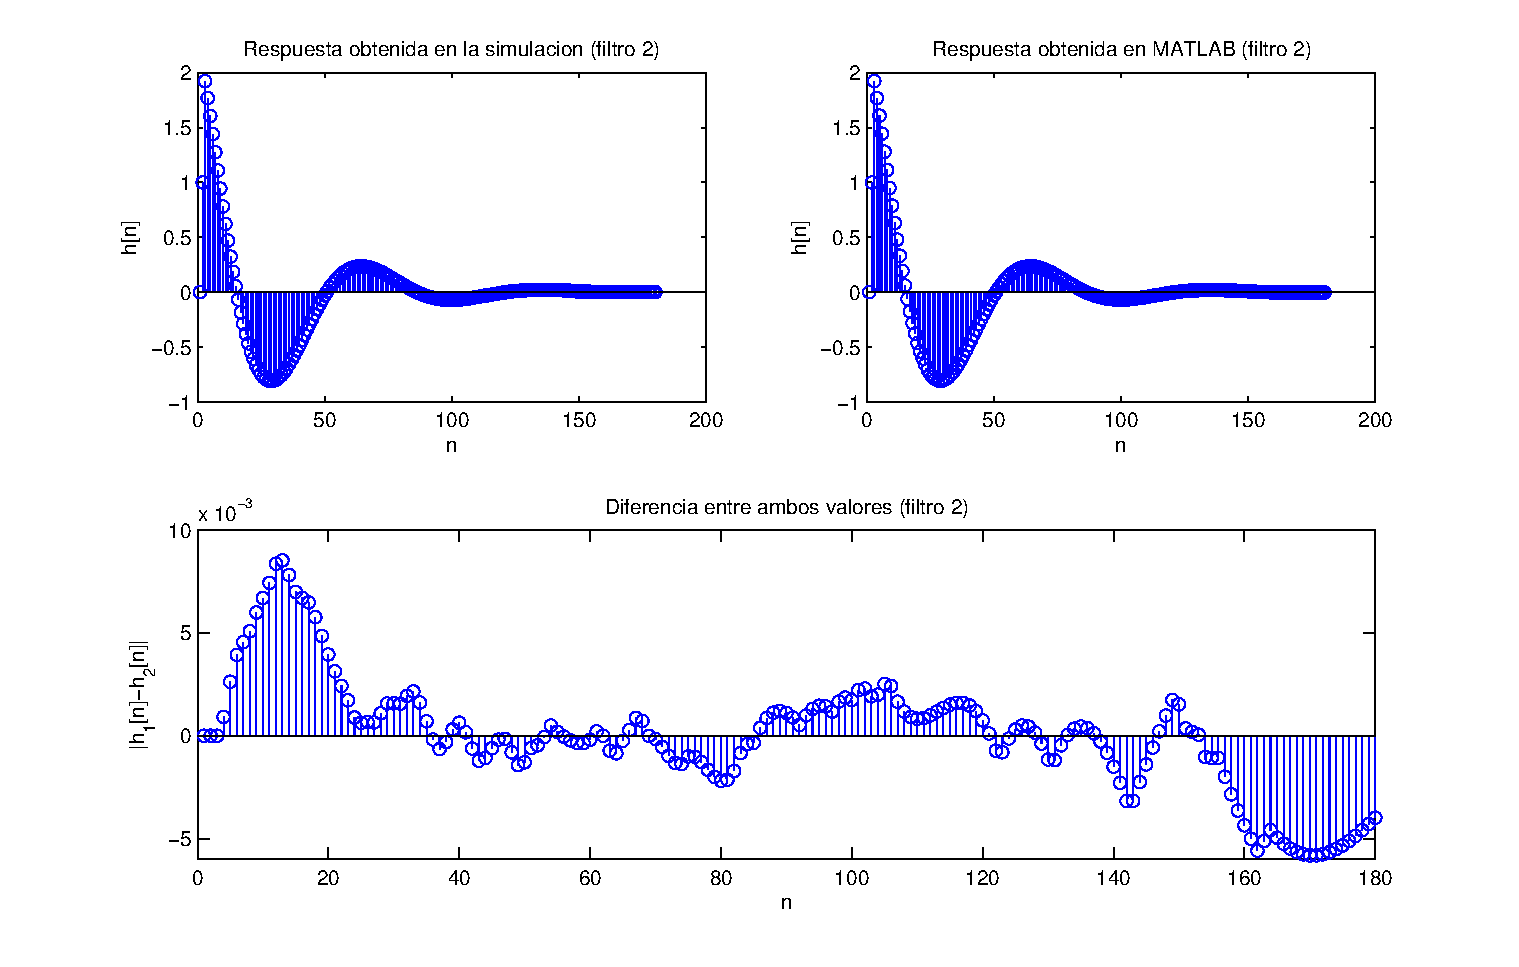
\includegraphics[width=\textwidth]{img/respfiltro2.pdf} 
\caption{Comprobación del filtro 2} \label{fig:filter2}
\end{figure}

\begin{figure}[hbt]
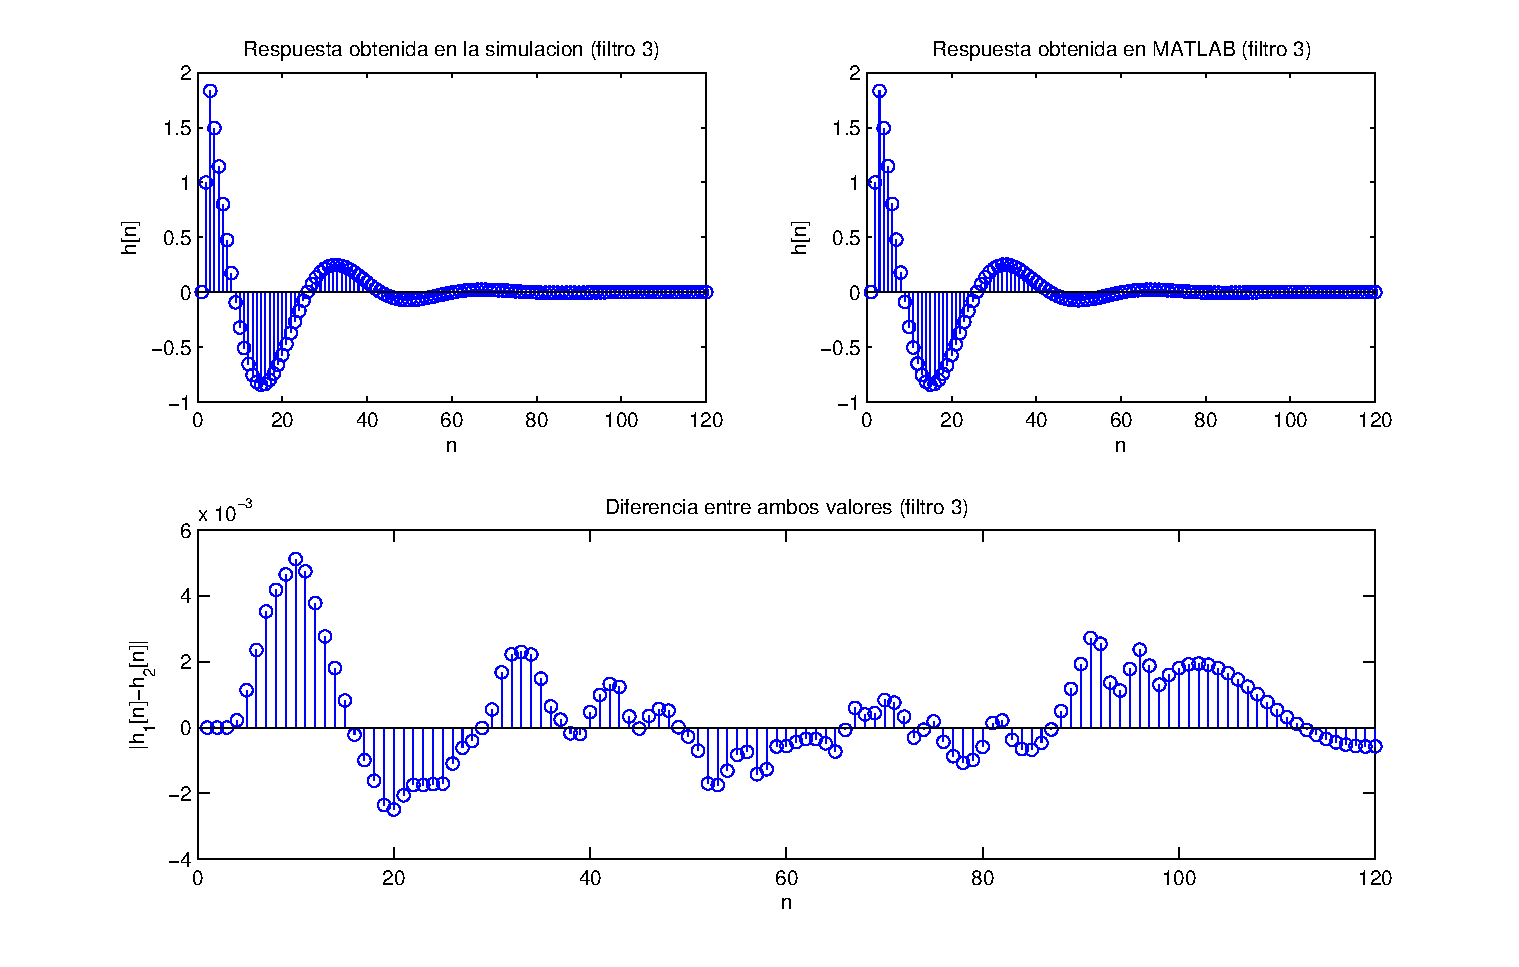
\includegraphics[width=\textwidth]{img/respfiltro3.pdf} 
\caption{Comprobación del filtro 3} \label{fig:filter3}
\end{figure}

\begin{figure}[hbt]
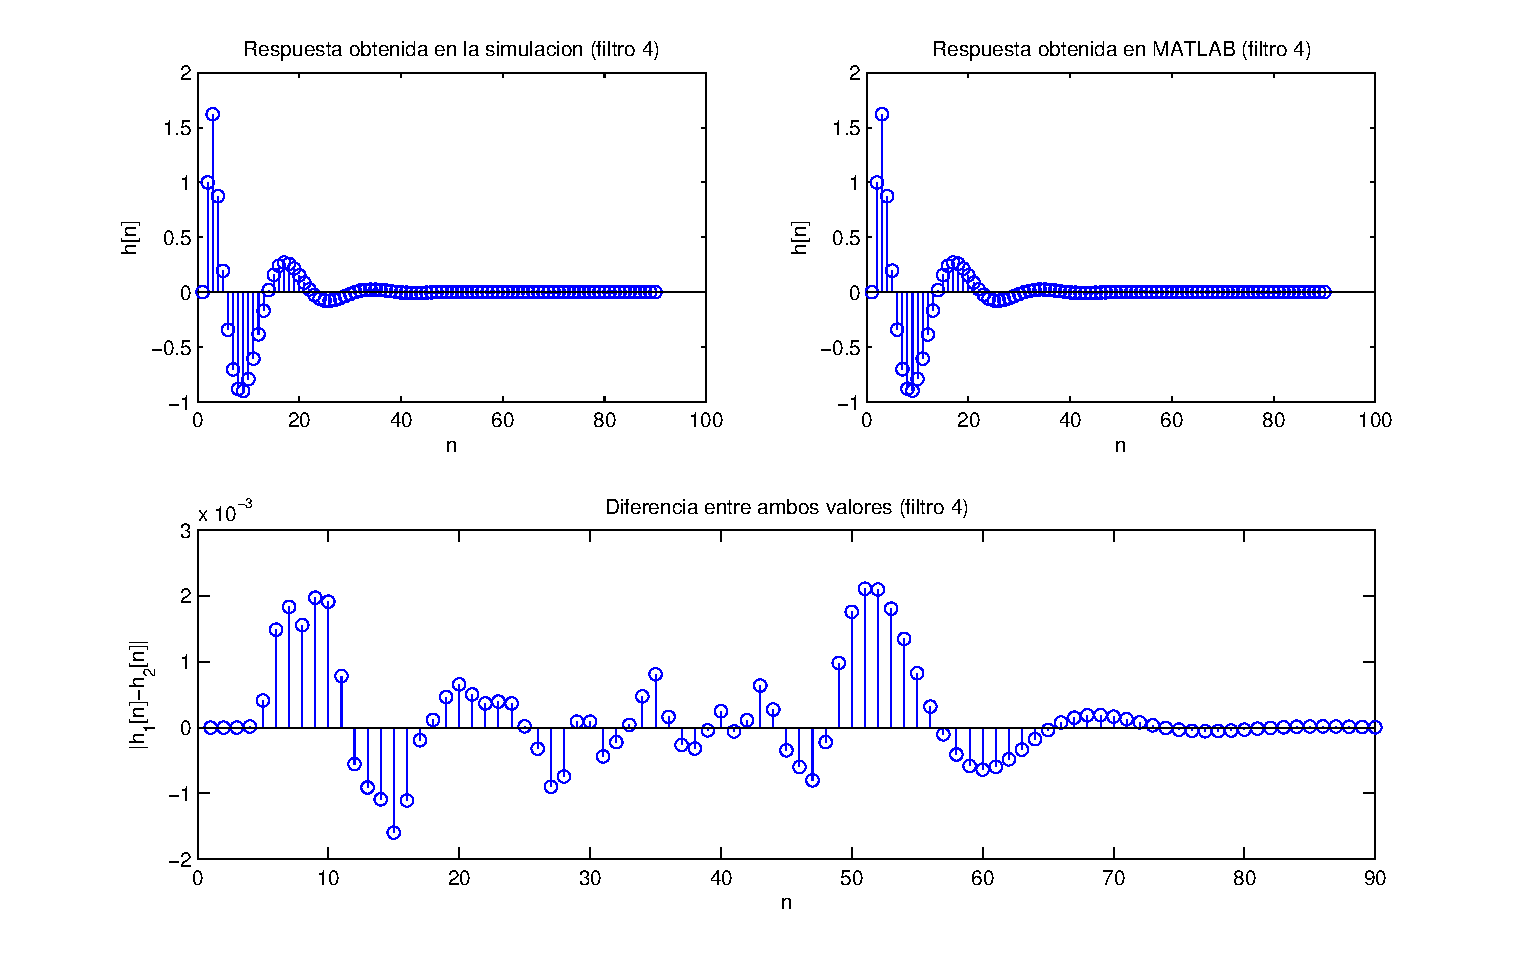
\includegraphics[width=\textwidth]{img/respfiltro4.pdf} 
\caption{Comprobación del filtro 4} \label{fig:filter4}
\end{figure}

\begin{figure}[hbt]
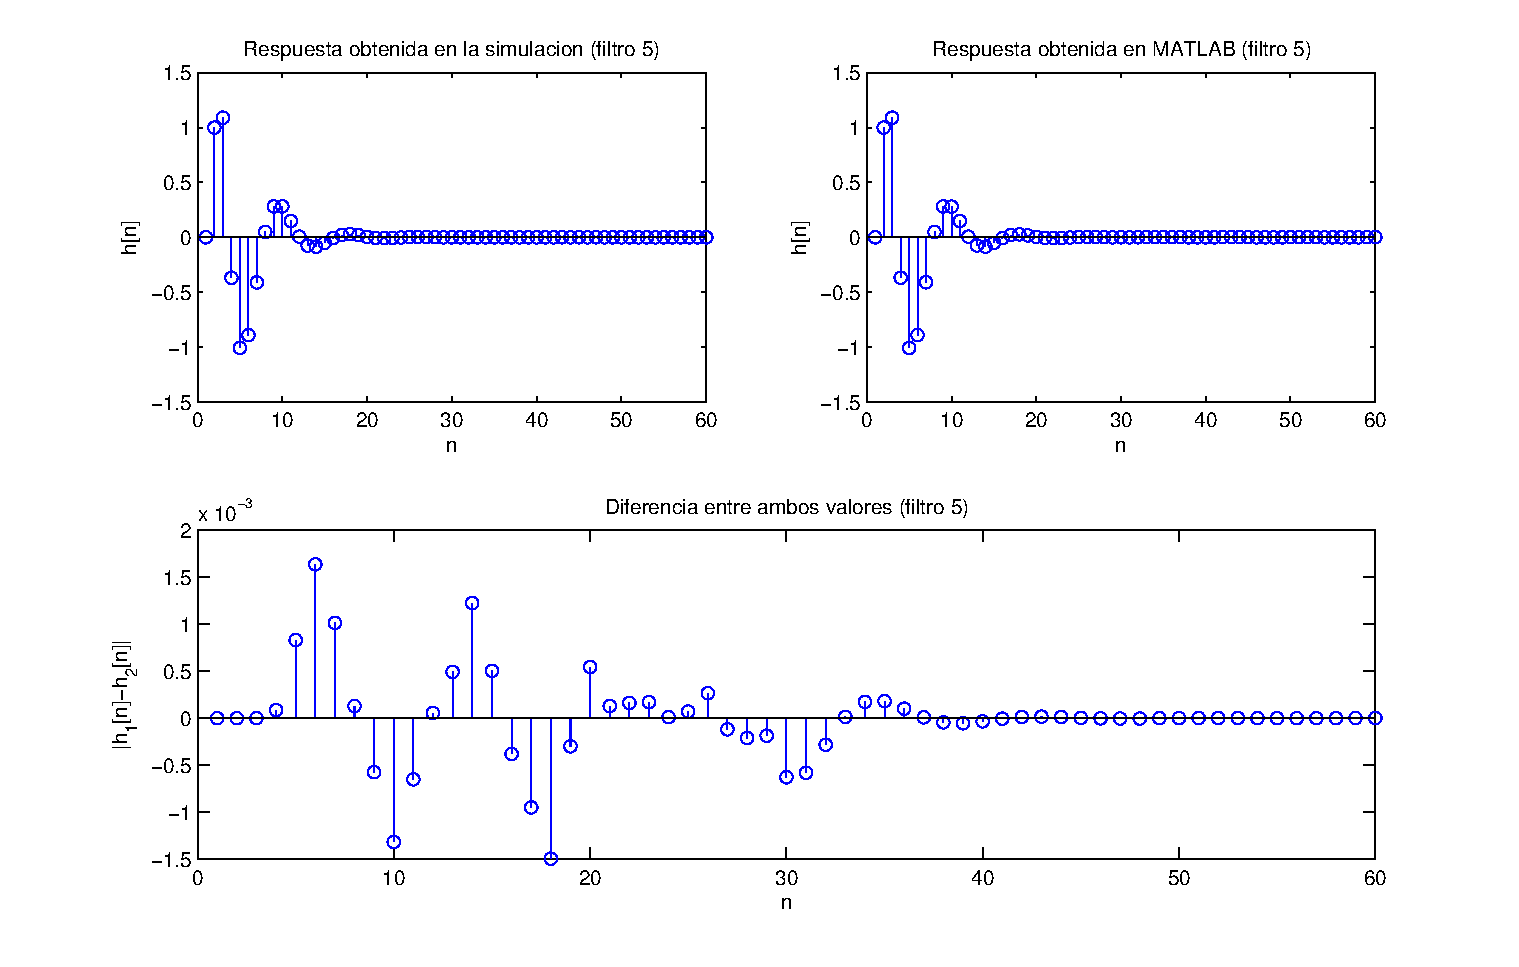
\includegraphics[width=\textwidth]{img/respfiltro5.pdf} 
\caption{Comprobación del filtro 5} \label{fig:filter5}
\end{figure}

\begin{figure}[hbt]
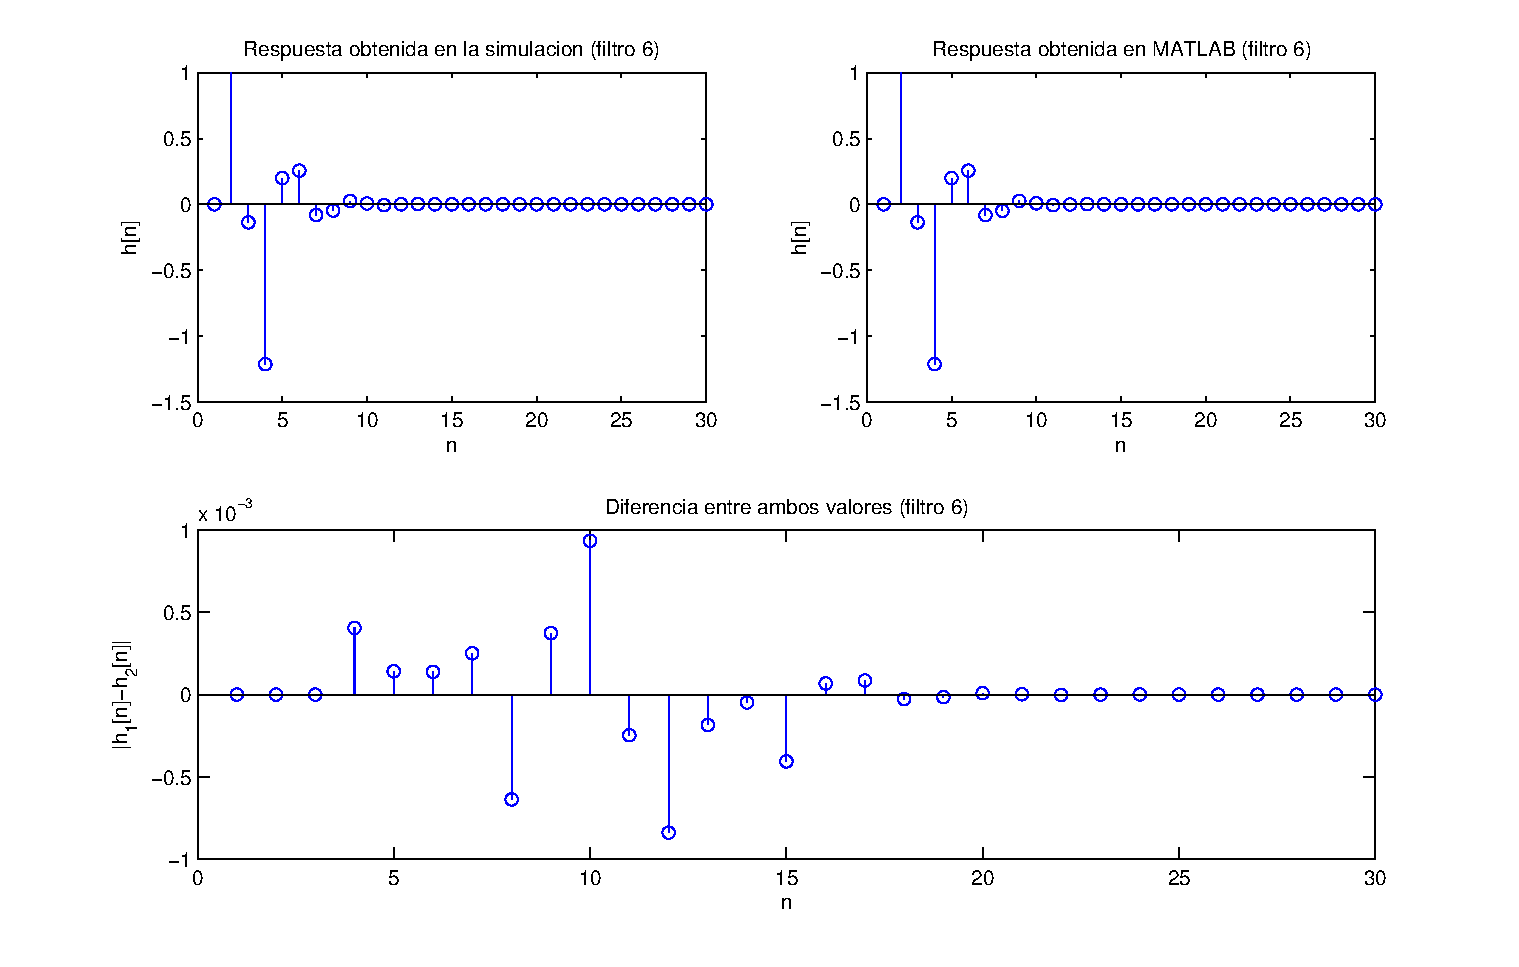
\includegraphics[width=\textwidth]{img/respfiltro6.pdf} 
\caption{Comprobación del filtro 6} \label{fig:filter6}
\end{figure}

\clearpage
\subsection{Aplicando atenuación}
\begin{figure}[hbt]
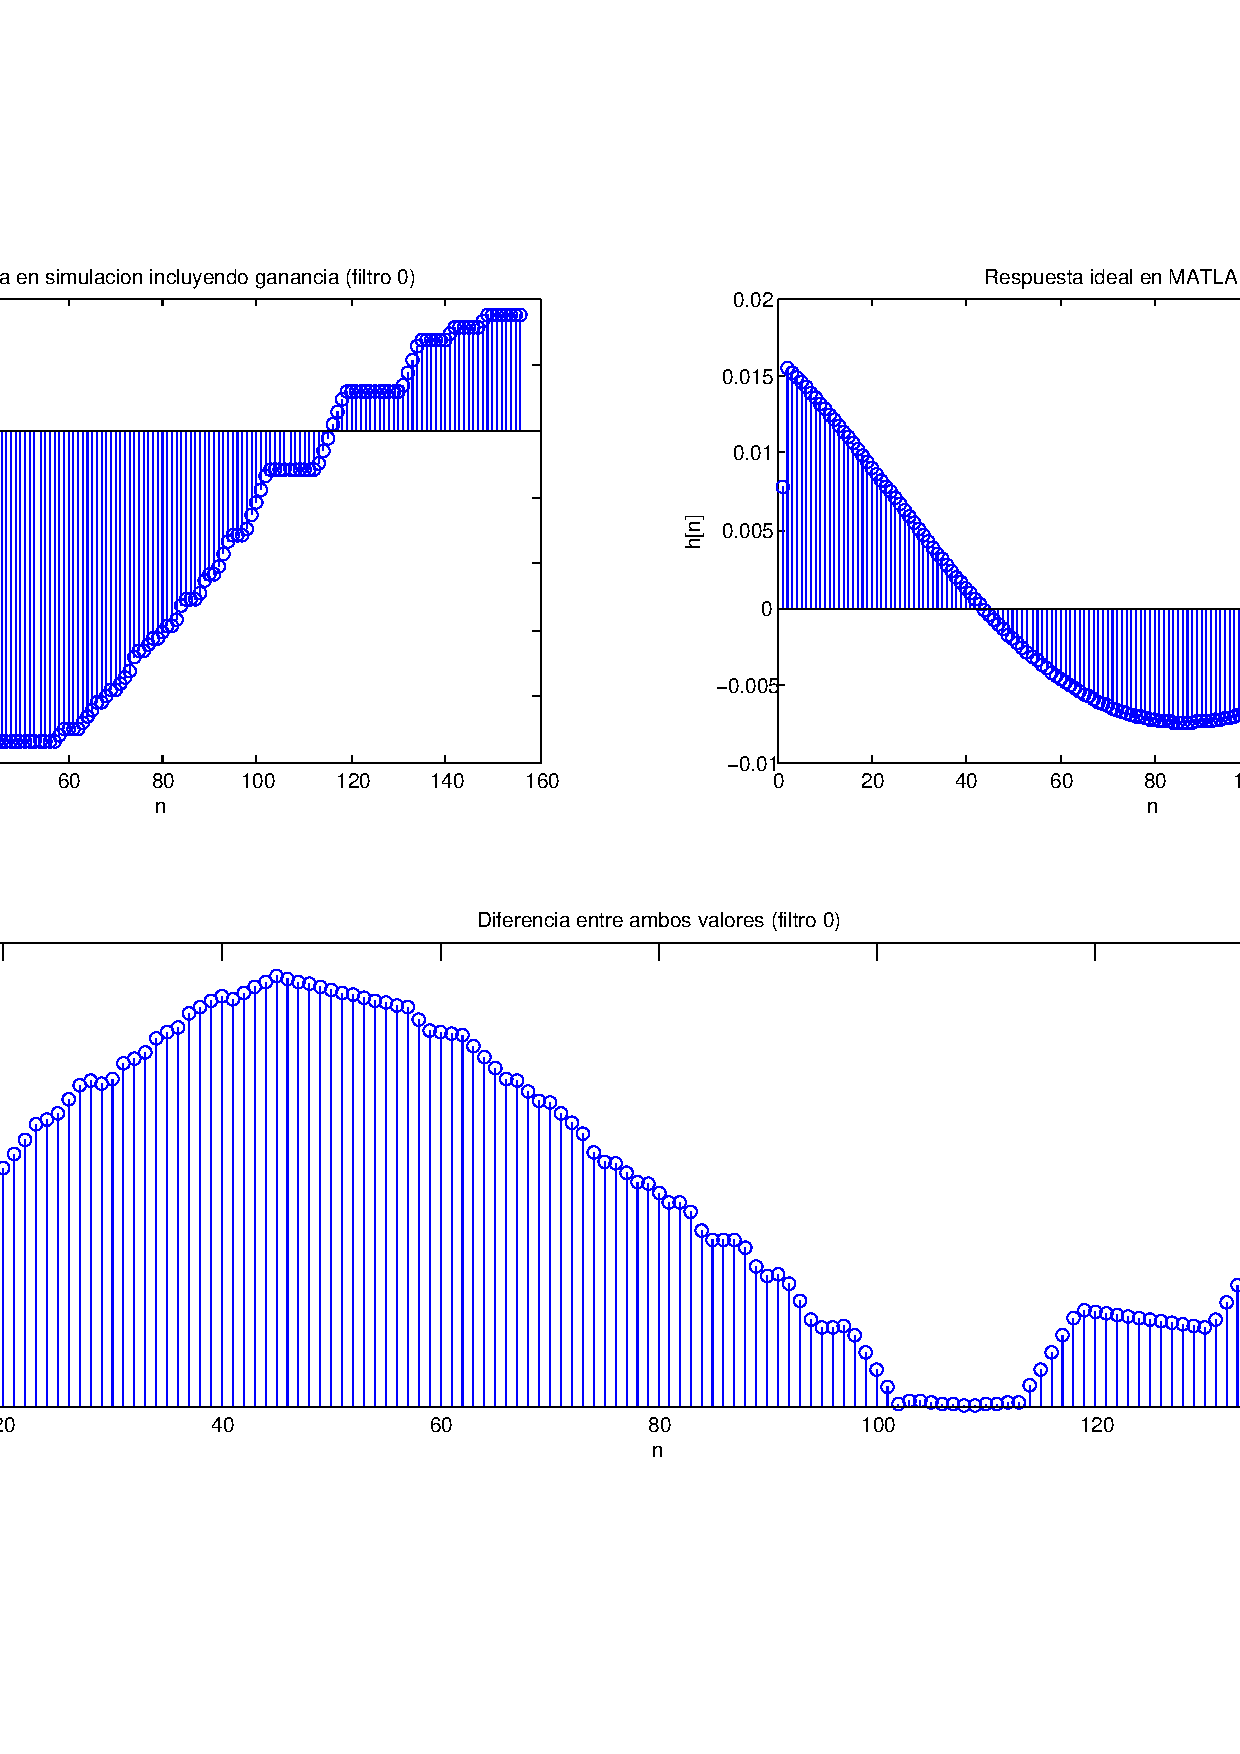
\includegraphics[width=\textwidth]{img/respfiltro0_gain.pdf} 
\caption{Comprobación del filtro 0 (con atenuación)} \label{fig:filter0_gain}
\end{figure}

\begin{figure}[hbt]
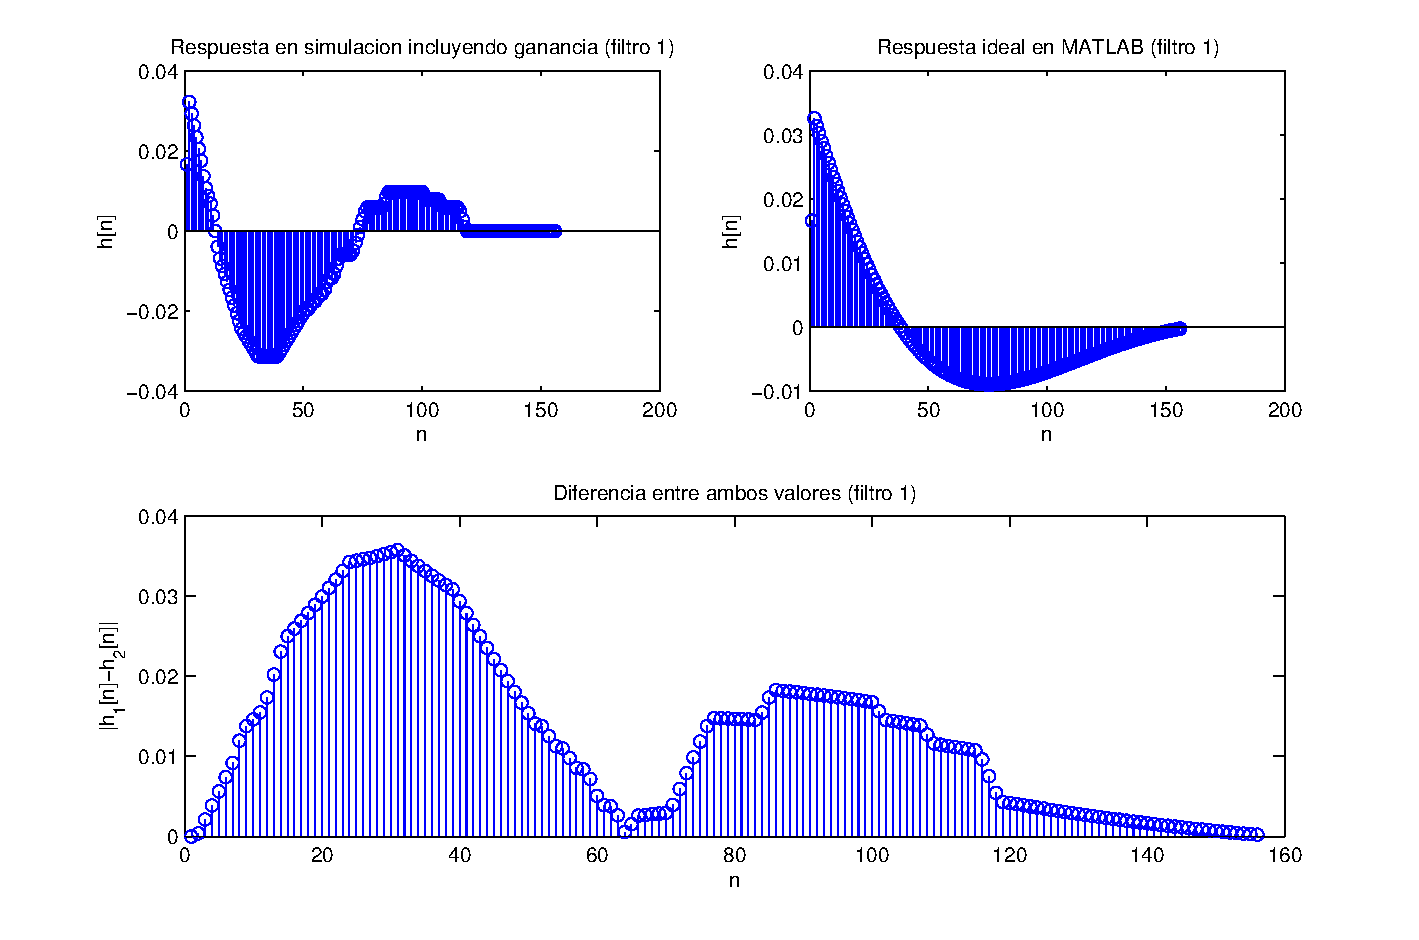
\includegraphics[width=\textwidth]{img/respfiltro1_gain.pdf} 
\caption{Comprobación del filtro 1 (con atenuación)} \label{fig:filter1_gain}
\end{figure}

\begin{figure}[hbt]
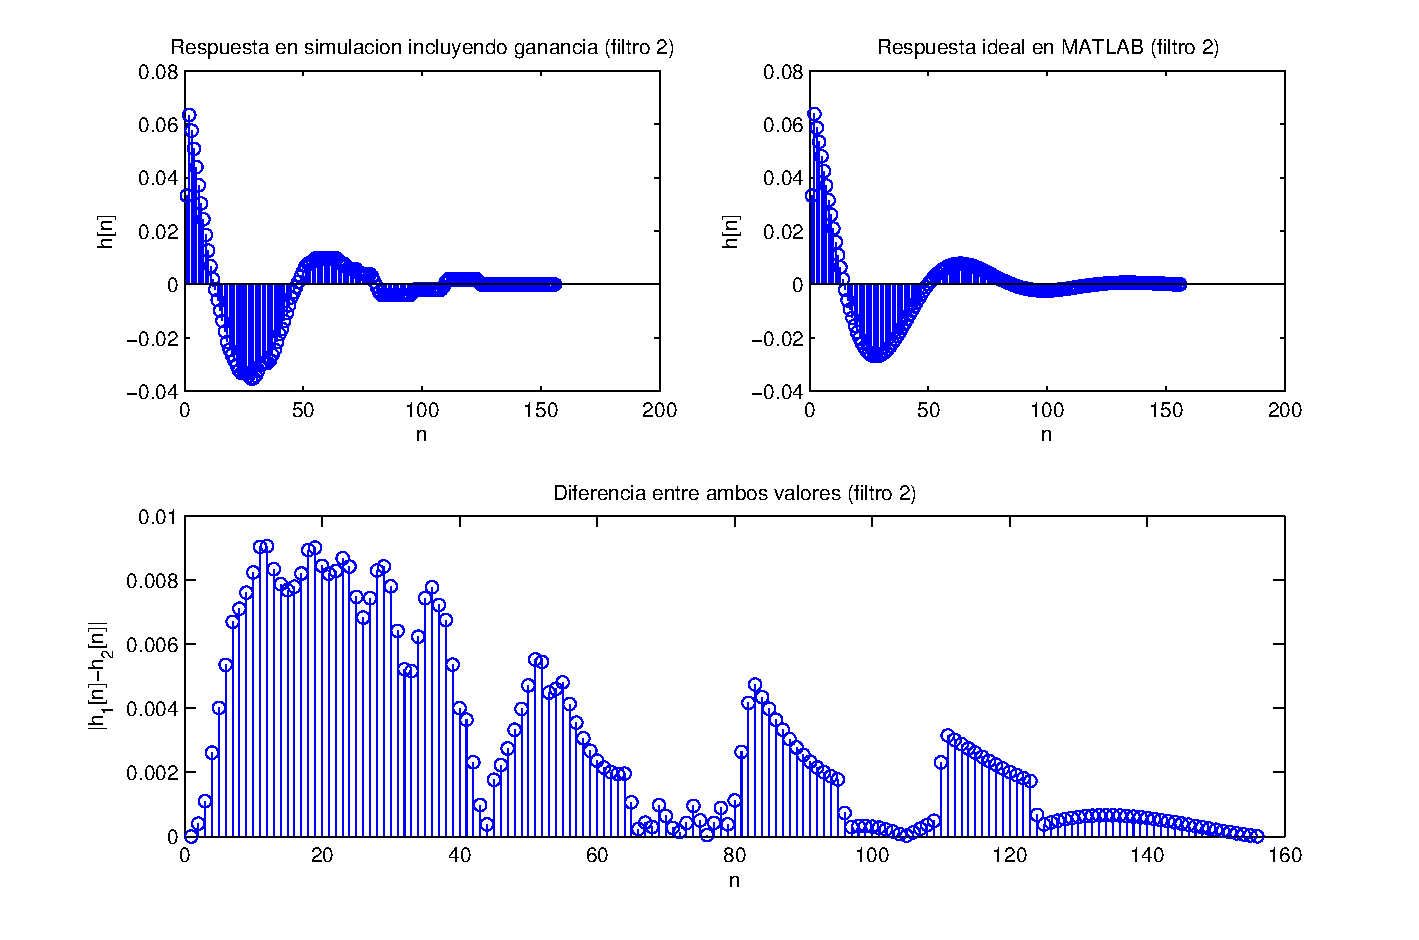
\includegraphics[width=\textwidth]{img/respfiltro2_gain.pdf} 
\caption{Comprobación del filtro 2 (con atenuación)} \label{fig:filter2_gain}
\end{figure}

\begin{figure}[hbt]
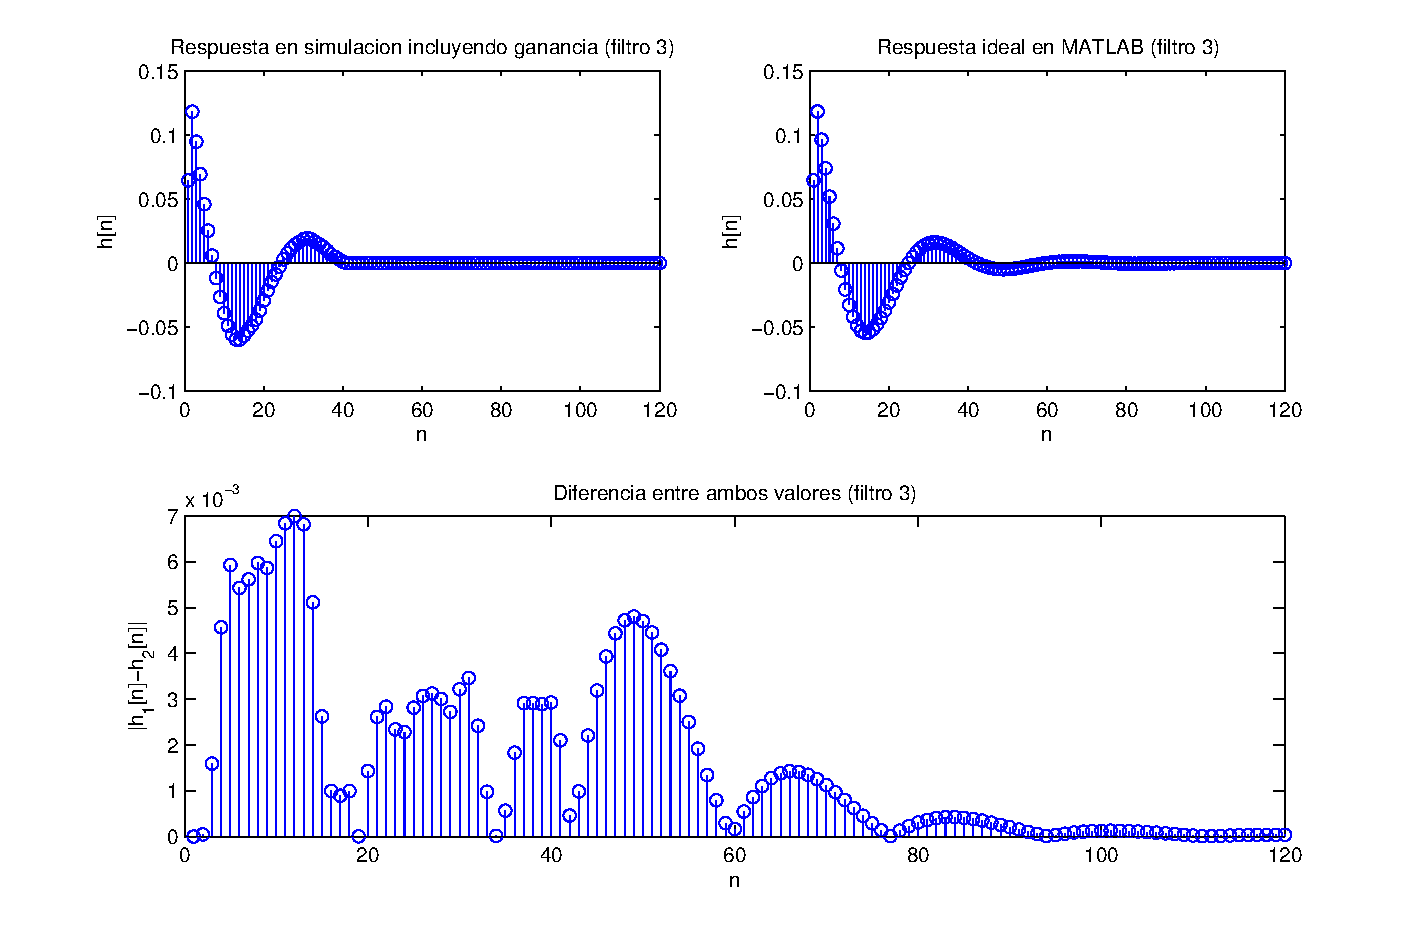
\includegraphics[width=\textwidth]{img/respfiltro3_gain.pdf} 
\caption{Comprobación del filtro 3 (con atenuación)} \label{fig:filter3_gain}
\end{figure}

\begin{figure}[hbt]
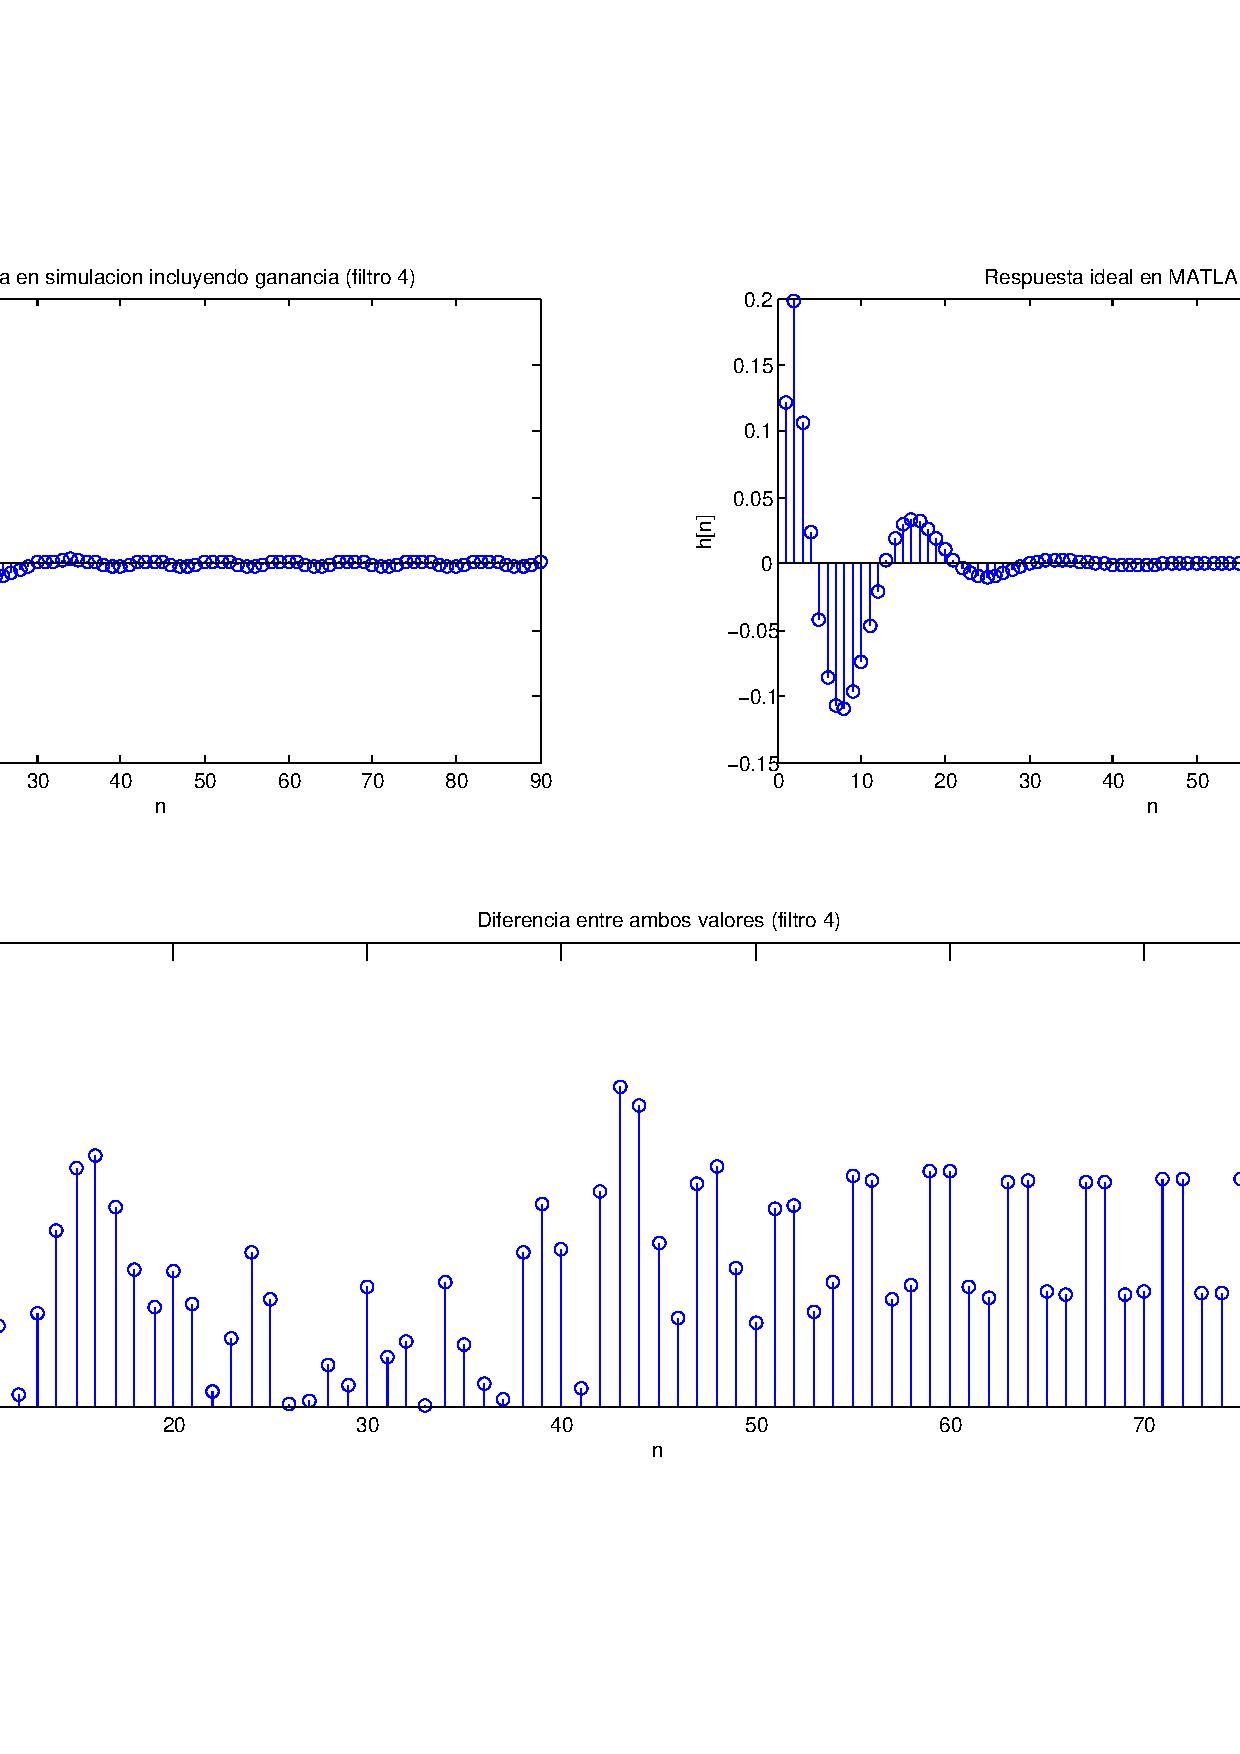
\includegraphics[width=\textwidth]{img/respfiltro4_gain.pdf} 
\caption{Comprobación del filtro 4 (con atenuación)} \label{fig:filter4_gain}
\end{figure}

\begin{figure}[hbt]
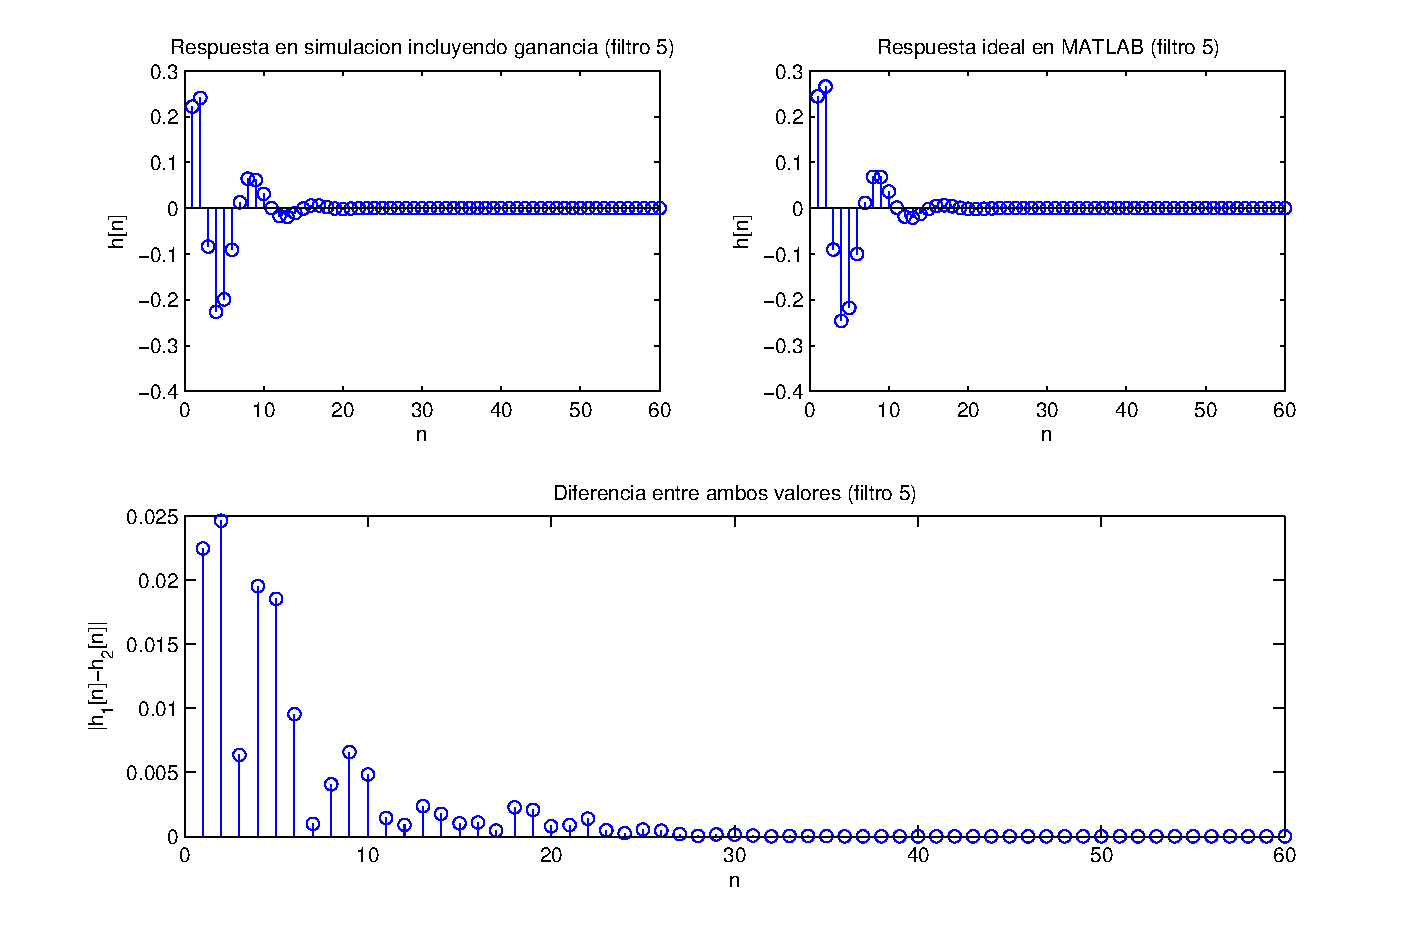
\includegraphics[width=\textwidth]{img/respfiltro5_gain.pdf} 
\caption{Comprobación del filtro 5 (con atenuación)} \label{fig:filter5_gain}
\end{figure}

\begin{figure}[hbt]
\begin{center}
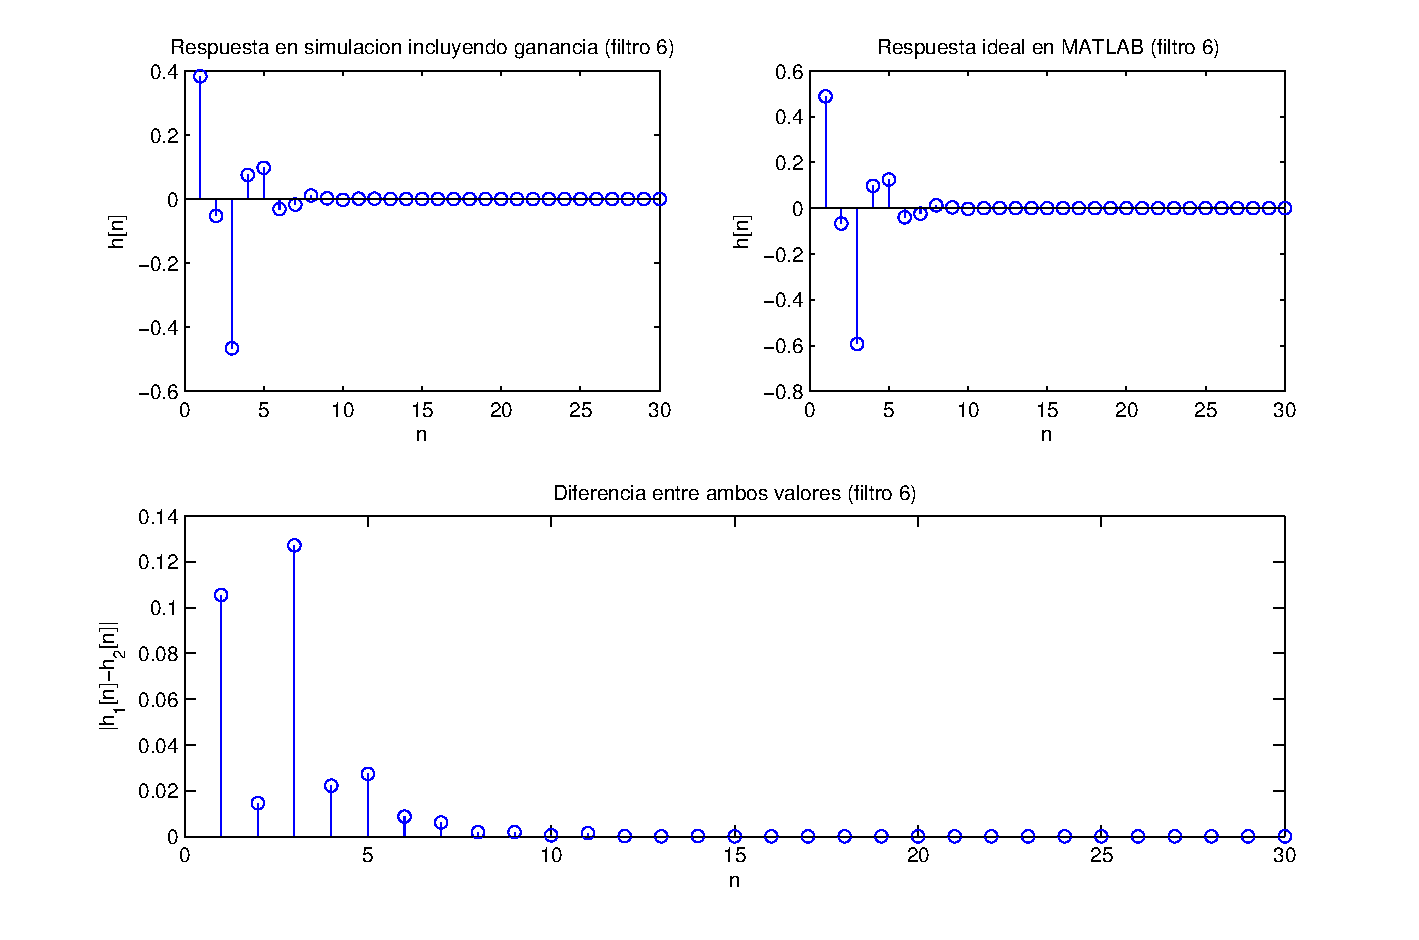
\includegraphics[width=\textwidth]{img/respfiltro6_gain.pdf} 
\caption{Comprobación del filtro 6 (con atenuación)} \label{fig:filter6_gain}
\end{center}
\end{figure}

\clearpage

\section{Gráficas de evaluación de reverb}\label{sec:resultadosreverb}
\begin{figure}[hbt]
\begin{center}
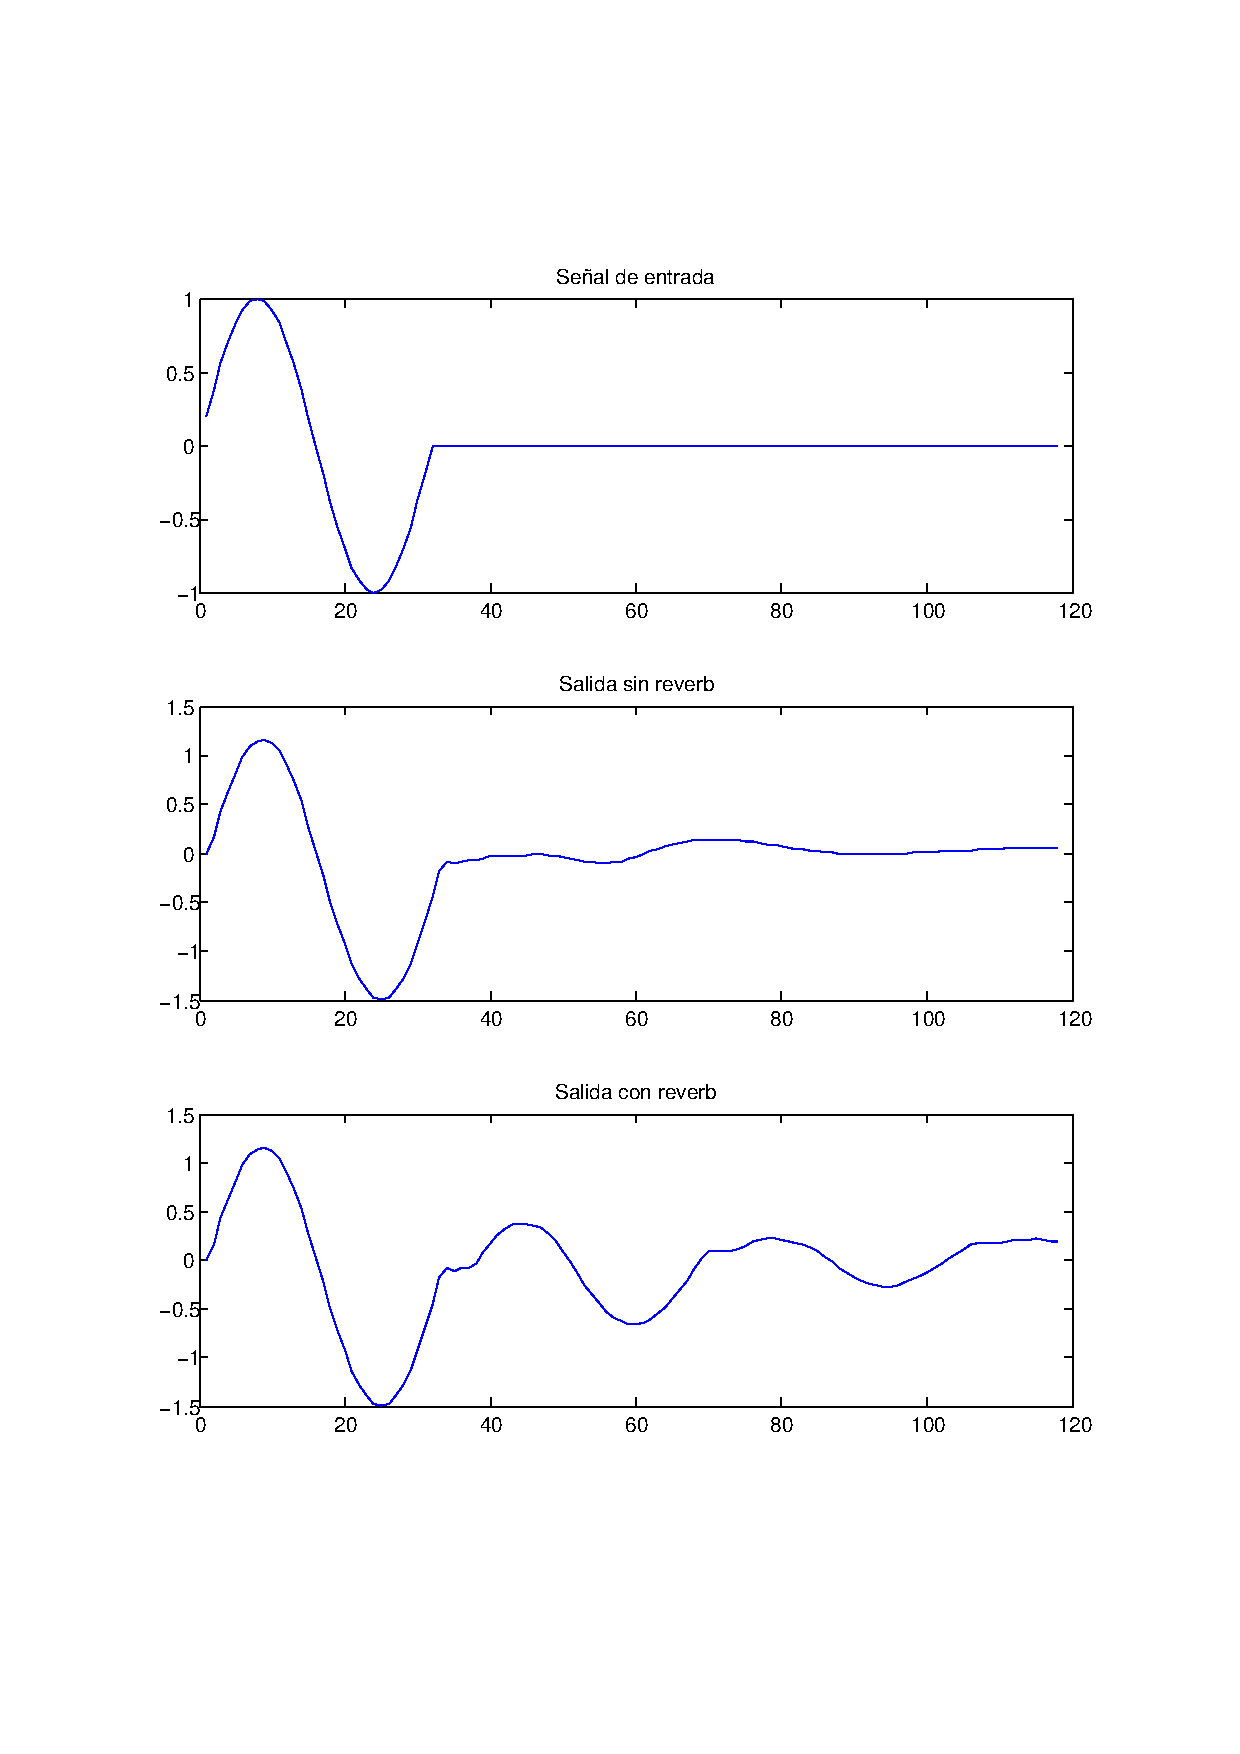
\includegraphics[width=10cm]{img/test_reverb.pdf} 
\caption{Comprobación de la función reverb} \label{fig:reverbgraph}
\end{center}
\end{figure}

\clearpage
\section{Gráficas de evaluación de ajuste de ganancia}\label{sec:resultadosajuste}
\begin{figure}[hbt]
\begin{center}
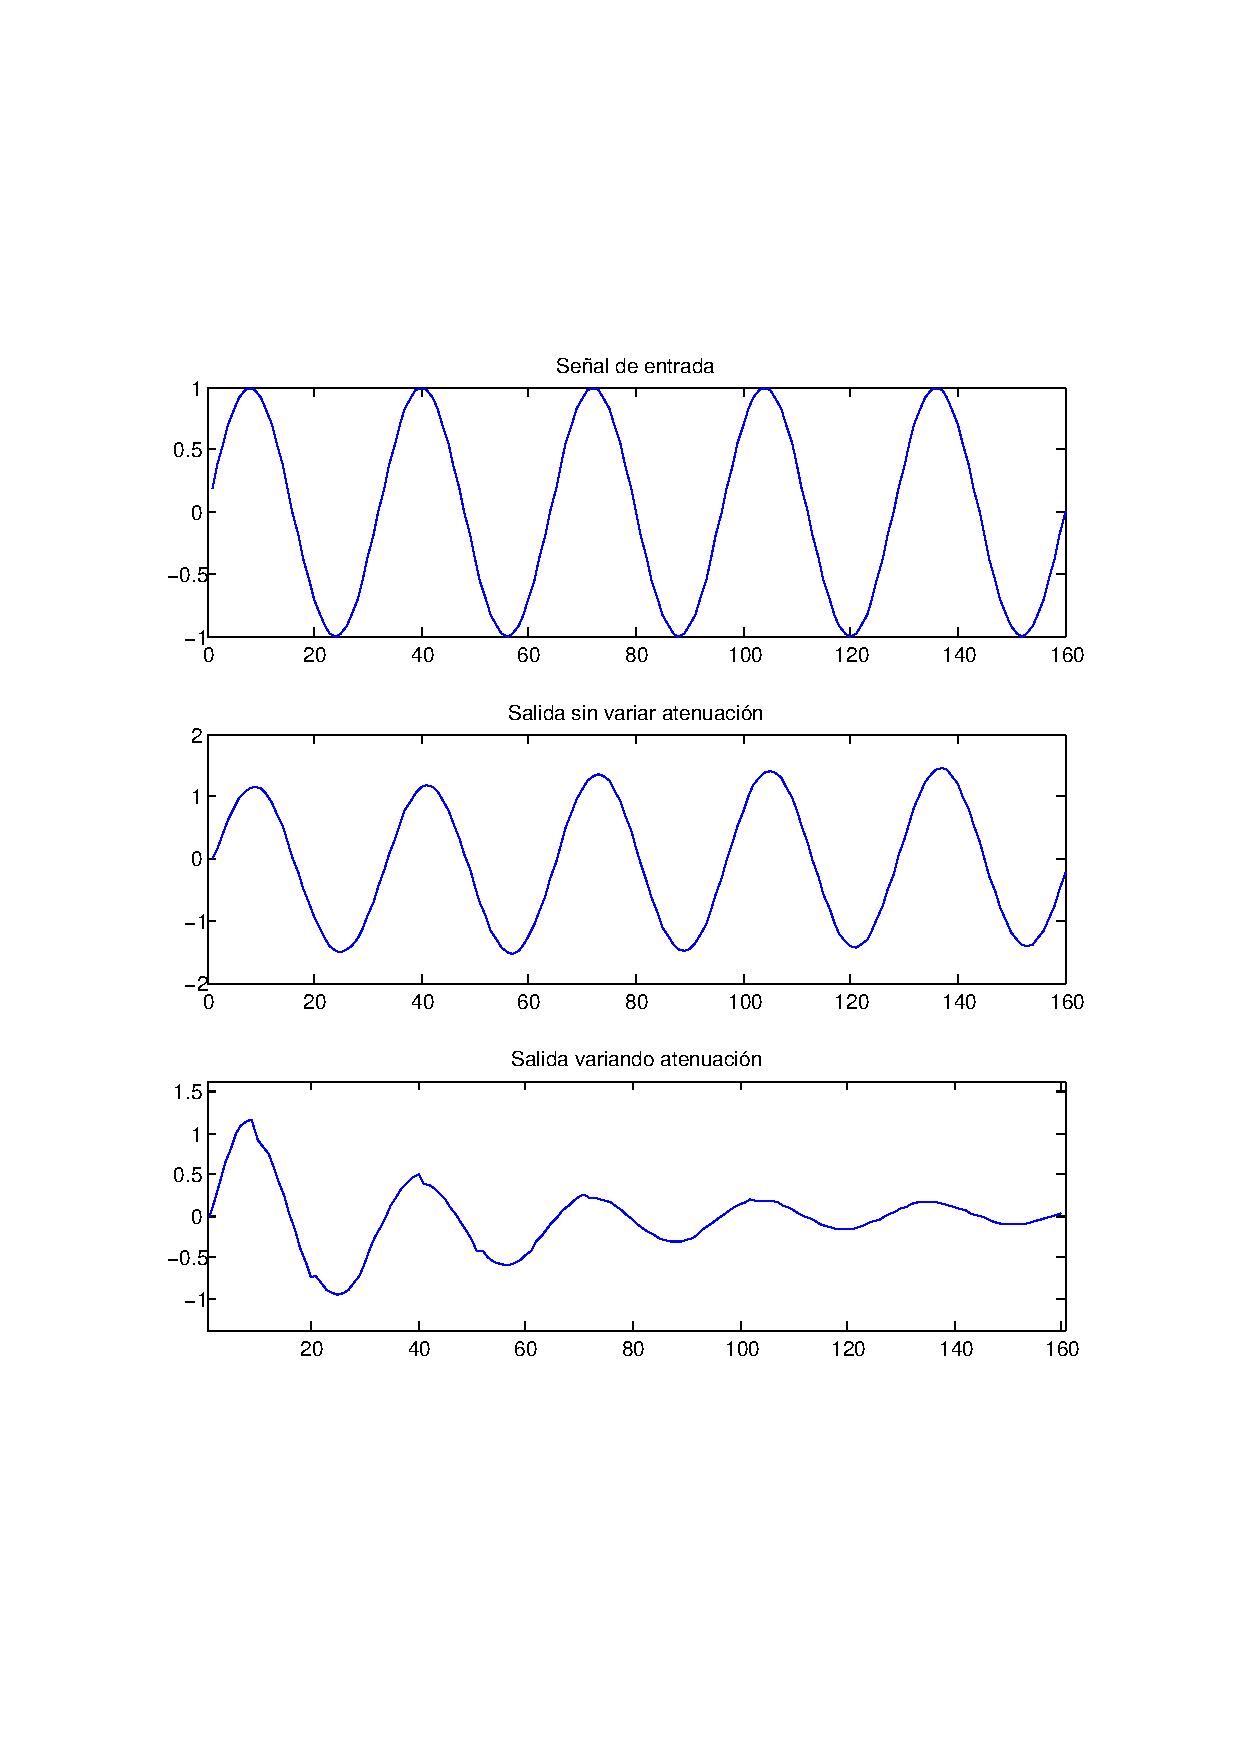
\includegraphics[width=10cm]{img/test_adjust.pdf} 
\caption{Comprobación del ajuste de ganancia} \label{fig:adjustgraph}
\end{center}
\end{figure}

\clearpage

\section{Gráficas de prueba de mejoras}\label{sec:resultadosmejoras}
\subsection{Sumadores}
En la gráfica que se presenta a continuación se pueden observar las siguientes señales:
\begin{description}
\item[Valid\_rc] Esta señal se pone a nivel alto cuando el resultado del sumador ripple carry es válido.
\item[Valid\_cb] Esta señal se pone a nivel alto cuando el resultado del sumador carry bypass es válido.
\item[sig1] Término 1 de la suma.
\item[sig2] Término 2 de la suma.
\item[sout\_rc] Resultado del sumador ripple carry.
\item[sout\_cb] Resultado del sumador carry bypass.
\item[sout\_ts] Resultado de la función + VHDL
\end{description}
En las señales valid\_rc y valid\_cb se observa la diferencia entre los tiempos de retardo de ambos sumadores.
\begin{figure}[hbt]
\begin{center}
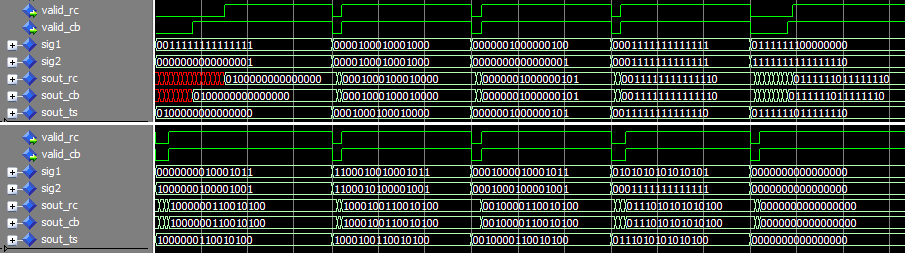
\includegraphics[width=\textwidth]{img/adder_test.png} 
\caption{Comprobación de sumadores} \label{fig:addertest}
\end{center}
\end{figure}

\subsection{Multiplicadores}
En la gráfica que se presenta a continuación se pueden observar las siguientes señales:
\begin{description}
\item[Valid\_ar] Esta señal se pone a nivel alto cuando el resultado del multiplicador en array es válido.
\item[Valid\_cs] Esta señal se pone a nivel alto cuando el resultado del multiplicador carry save es válido.
\item[signal1] Factor de la multiplicación.
\item[signal2] Factor de la multiplicación.
\item[mult\_cs] Resultado del multiplicador carry save.
\item[mult\_ar] Resultado del multiplicador en array.
\item[mult\_test] Resultado de la función * VHDL
\end{description}
En las señales valid\_ar y valid\_cs se observa la diferencia entre los tiempos de retardo de ambos multiplicadores.
\begin{figure}[hbt]
\begin{center}
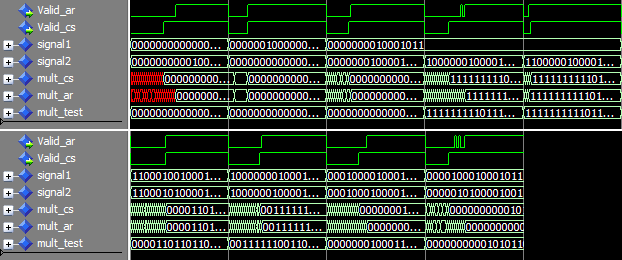
\includegraphics[width=\textwidth]{img/multiplier_test.png} 
\caption{Comprobación de multiplicadores} \label{fig:multipliertest}
\end{center}
\end{figure}


\end{document}
